% Тип документа
\documentclass[a4paper,14pt]{extarticle}

% Шрифты, кодировки, символьные таблицы, переносы
\usepackage{cmap}
\usepackage[T2A]{fontenc}
\usepackage[utf8x]{inputenc}
\usepackage[russian]{babel}

% Это пакет -- хитрый пакет, он нужен но не нужен
\usepackage[mode=buildnew]{standalone}

\usepackage
	{
		% Дополнения Американского математического общества (AMS)
		amssymb,
		amsfonts,
		amsmath,
		% amsthm,
		% misccorr,
		% 
		% Графики и рисунки
		wrapfig,
		graphicx,
		subcaption,
		float,
		tikz,
		tikz-3dplot,
		caption,
		csvsimple,
		color,
		booktabs,
		pgfplots,
		pgfplotstable,
		geometry,
		% 
		% Таблицы, списки
		makecell,
		multirow,
		indentfirst,
		%
		% Интегралы и прочие обозначения
		ulem,
		esint,
		esdiff,
		% 
		% Колонтитулы
		fancyhdr,
	}  


% Обводка текста в TikZ
\usepackage[outline]{contour}

% Увеличенный межстрочный интервал, французские пробелы
% \linespread{1.3} 
\frenchspacing 

 
\usetikzlibrary
	{
		decorations.pathreplacing,
		decorations.pathmorphing,
		patterns,
		calc,
		scopes,
		arrows,
		fadings,
		through,
		shapes.misc,
		arrows.meta,
		3d,
		quotes,
		angles,
		babel
	}


\tikzset{
	force/.style=	{
		>=latex,
		draw=blue,
		fill=blue,
				 	}, 
	%				 	
	axis/.style=	{
		densely dashed,
		blue,
		line width=1pt,
		font=\small,
					},
	%
	th/.style=	{
		line width=1pt},
	%
	acceleration/.style={
		>=open triangle 60,
		draw=magenta,
		fill=magenta,
					},
	%
	inforce/.style=	{
		force,
		double equal sign distance=2pt,
					},
	%
	interface/.style={
		pattern = north east lines, 
		draw    = none, 
		pattern color=gray!60,
					},
	cross/.style=	{
		cross out, 
		draw=black, 
		minimum size=2*(#1-\pgflinewidth), 
		inner sep=0pt, outer sep=0pt,
					},
	%
	cargo/.style=	{
		rectangle, 
		fill=black!70, 
		inner sep=2.5mm,
					},
	%
	caption/.style= {
		midway,
		fill=white!20, 
		opacity=0.9
					},
	%
	}

\newenvironment{tikzpict}
    {
	    \begin{figure}[htbp]
		\centering
		\begin{tikzpicture}
    }
    { 
		\end{tikzpicture}
		% \caption{caption}
		% \label{fig:label}
		\end{figure}
    }


\newcommand{\vbLabel}[3]{\draw ($(#1,#2)+(0,5pt)$) -- ($(#1,#2)-(0,5pt)$) node[below]{#3}}
\newcommand{\vaLabel}[3]{\draw ($(#1,#2)+(0,5pt)$) node[above]{#3} -- ($(#1,#2)-(0,5pt)$) }

\newcommand{\hrLabel}[3]{\draw ($(#1,#2)+(5pt,0)$) -- ($(#1,#2)-(5pt,0)$) node[right, xshift=1em]{#3}}
\newcommand{\hlLabel}[3]{\draw ($(#1,#2)+(5pt,0)$) node[left, xshift=-1em]{#3} -- ($(#1,#2)-(5pt,0)$) }



\newcommand\zi{^{\,*}_i}
\newcommand\sumn{\sum_{i=1}^{N}}

\tikzset{
	coordsys/.style={scale=1.8,x={(1.1cm,-0cm)},y={(0.5cm,1cm)}, z={(0cm,0.8cm)}},
	coordsys/.style={scale=1.5,x={(0cm,0cm)},y={(1cm,0cm)}, z={(0cm,1cm)}}, 
	coordsys/.style={scale=1.5,x={(1cm,0cm)},y={(0cm,1cm)}, z={(0cm,0cm)}}, 
}

\usepgfplotslibrary{units}


% Draw line annotation
% Input:
%   #1 Line offset (optional)
%   #2 Line angle
%   #3 Line length
%   #5 Line label
% Example:
%   \lineann[1]{30}{2}{$L_1$}

\newcommand{\lineann}[4][0.5]{%
    \begin{scope}[rotate=#2, blue,inner sep=2pt, ]
        \draw[dashed, blue!40] (0,0) -- +(0,#1)
            node [coordinate, near end] (a) {};
        \draw[dashed, blue!40] (#3,0) -- +(0,#1)
            node [coordinate, near end] (b) {};
        \draw[|<->|] (a) -- node[fill=white, scale=0.8] {#4} (b);
    \end{scope}
}

\newcommand{\lineannn}[4][0.5]{%
    \begin{scope}[rotate=#2, blue,inner sep=2pt, ]
        \draw[dashed, blue!40] (0,0) -- +(0,#1)
            node [coordinate, near end] (a) {};
        \draw[dashed, blue!40] (#3,0) -- +(0,#1)
            node [coordinate, near end] (b) {};
        % \draw[color=white, color=blue] (a) -- node[fill=white, scale=0.8] {#4} (b);
        \draw[->|] (a)++(-0.3,0) -- (a);
        \draw[->|] (b)++(0.3,0) coordinate (xx) -- (b);
        \draw (xx) node[fill=white, scale=0.8, right] {#4};
    \end{scope}
}

% Круговая стрелка относительно центра (дуга из центра)
\tikzset{
  pics/carc/.style args={#1:#2:#3}{
    code={
      \draw[pic actions] (#1:#3) arc(#1:#2:#3);
    }
  },
  dash/.style={
  	dash pattern=on 5mm off 5mm
  }
}

% Среднее <#1>
\newcommand{\mean}[1]{\langle#1\rangle}

\pgfplotsset{
    % most recent feature set of pgfplots
    compat=newest,
}

% const прямым шрифтом
\newcommand\ct[1]{\text{\rmfamily\upshape #1}}
\newcommand*{\const}{\ct{const}}


\usepackage[europeanresistors,americaninductors]{circuitikz}

% Style to select only points from #1 to #2 (inclusive)
\pgfplotsset{select/.style 2 args={
    x filter/.code={
        \ifnum\coordindex<#1\def\pgfmathresult{}\fi
        \ifnum\coordindex>#2\def\pgfmathresult{}\fi
    }
}}


\usepackage{array}



%%%%%%%%%%%%%%%%%%%%%%%%%%%%%%%%%%%%%%%%%%%%%%%%%
\makeatletter
\newif\if@gather@prefix 
\preto\place@tag@gather{% 
  \if@gather@prefix\iftagsleft@ 
    \kern-\gdisplaywidth@ 
    \rlap{\gather@prefix}% 
    \kern\gdisplaywidth@ 
  \fi\fi 
} 
\appto\place@tag@gather{% 
  \if@gather@prefix\iftagsleft@\else 
    \kern-\displaywidth 
    \rlap{\gather@prefix}% 
    \kern\displaywidth 
  \fi\fi 
  \global\@gather@prefixfalse 
} 
\preto\place@tag{% 
  \if@gather@prefix\iftagsleft@ 
    \kern-\gdisplaywidth@ 
    \rlap{\gather@prefix}% 
    \kern\displaywidth@ 
  \fi\fi 
} 
\appto\place@tag{% 
  \if@gather@prefix\iftagsleft@\else 
    \kern-\displaywidth 
    \rlap{\gather@prefix}% 
    \kern\displaywidth 
  \fi\fi 
  \global\@gather@prefixfalse 
} 
\newcommand*{\beforetext}[1]{% 
  \ifmeasuring@\else
  \gdef\gather@prefix{#1}% 
  \global\@gather@prefixtrue 
  \fi
} 
\makeatother
%%%%%%%%%%%%%%%%%%%%%%%%%%%%%%%%%%%%%%%%%%%%%%%%%

\geometry		
	{
		left			=	2cm,
		right 			=	2cm,
		top 			=	3cm,
		bottom 			=	3cm,
		bindingoffset	=	0cm
	}

%%%%%%%%%%%%%%%%%%%%%%%%%%%%%%%%%%%%%%%%%%%%%%%%%%%%%%%%%%%%%%%%%%%%%%%%%%%%%%%



	%применим колонтитул к стилю страницы

%%%%%%%%%%%%%%%%%%%%%%%%%%%%%%%%%%%%%%%%%%%%%%%%%%%%%%%%%%%%%%%%%%%%%%%%%%%%%%%

\renewcommand{\contentsname}{Оглавление}

\usepackage{tocloft}
% \renewcommand{\cftpartleader}{\cftdotfill{\cftdotsep}} % for parts
% \renewcommand{\cftsectiondotsep}{\cftdotsep}% Chapters should use dots in ToC
\renewcommand{\cftsecleader}{\cftdotfill{\cftdotsep}}
%\renewcommand{\cftsecleader}{\cftdotfill{\cftdotsep}} % for sections, if you really want! (It is default in report and book class (So you may not need it).
% ---------
% \newcommand{\cftchapaftersnum}{.}%
% \usepackage{titlesec}
% \titlelabel{\thetitle.\quad}
\usepackage{secdot}
\sectiondot{subsection}
\usepackage{setspace}
\usepackage{amsmath, amssymb}
\newcommand{\noo}{\varnothing}
\usepackage{amsthm}
\DeclareMathOperator{\sinc}{sinc}
% \newcommand{\dif}[3]{

% \newtheorem{mydef}{}
\newtheorem{mydef}{Определение}[section]
% \newtheorem{ppp}{Предложение}

% <<<<<<< Updated upstream
\newtheorem{theorem}{Теорема}[section]

\newtheorem{lemma}[theorem]{Лемма}%[section]

\theoremstyle{definition}
\newtheorem{consq}[theorem]{Следствие}%[section]
\newtheorem{definition}[theorem]{Определение}%[section]
\newtheorem{deflemma}[theorem]{Лемма-определение}%[section]
\newtheorem{zam}[theorem]{Замечание}
% \newtheorem{lemma}{Лемма}

\theoremstyle{remark}
\newtheorem{remark}[theorem]{Замечание}%[section]

\pagestyle{fancy} 
	%очистим "шапку" страницы
\fancyhead{} 
	%слева сверху на четных и справа на нечетных
\fancyhead[R]{Теория вероятностей} 
	%справа сверху на четных и слева на нечетных
\fancyhead[L]{Методичка} 
	%очистим "подвал" страницы
\fancyfoot{} 
	% номер страницы в нижнем колинтуле в центре
\fancyfoot[C]{\thepage} 

\newcommand{\ssm}{\smallsetminus}
\renewcommand{\O}{\noo}
\renewcommand{\backslash}{\smallsetminus}

% \theoremstyle{definition}
% \theoremstyle{theorem}
% \newtheorem{theorem}[definition]{Теорема}

\begin{document}


\def\labauthors{}
\def\labgroup{}
\def\labnumber{}
\def\labtheme{}
\renewcommand{\vec}{\mathbf}
\renewcommand{\Re}{\operatorname{Re}}
\renewcommand{\Im}{\operatorname{Im}}
\renewcommand{\phi}{\varphi}
\renewcommand{\kappa}{\varkappa}
\renewcommand{\hat}{\widehat}
%%%%%%%%%%%%%%%%%%%%%%%%%%%%%%%%%%%%%%%%%%%%%%%%%%%%%%%%%%%%%%%%%%%%%%%%%%%%%%%
% %!TEX root = ../var.tex
\begin{titlepage}

\begin{center}

{\small\textsc{Нижегородский государственный университет имени Н.\,И. Лобачевского}}
\vskip 1pt \hrule \vskip 3pt
{\small\textsc{Радиофизический факультет}}

\vfill

{ \LargeМетодическое пособие \vskip 12pt\bfseries \Huge Теория вероятностей}
	
\end{center}

\vfill
	
% \begin{flushright}
% 	{Выполнили студенты \labgroup\ группы\\ \labauthors}%\vskip 12pt Принял:\\ Менсов С.\,Н.}
% \end{flushright}
	
\vfill
	
\begin{center}
	Нижний Новгород, \the\year
\end{center}

\end{titlepage}

/
%%%%%%%%%%%%%%%%%%%%%%%%%%%%%%%%%%%%%%%%%%%%%%%%%%%%%%%%%%%%%%%%%%%%%%%%%%%%%%%
\begin{spacing}{1}
\tableofcontents
\end{spacing}
% \setstretch{1.2}
\newpage
\part*{Исторические сведения}
%!TEX root = ../var.tex

Возникновение теории вероятностей как науки относят к средним векам, когда появилась возможность и возникла необходимость изучения математическими методами азартных игр (таких как орлянка, кости, рулетка). 

Самые ранние работы учёных в области теории вероятностей относятся к XVII веку. Первоначально её основные понятия не имели строго математического описания. Задачи, из которых позже выросла теория вероятностей представляли набор некоторых эмпирических фактов о свойствах реальных событий, которые формулировались с помощью наглядных описаний. 

Исследуя прогнозирование выигрыша при бросании костей в письмах друг другу, Блез Паскаль и Пьер Ферма открыли первые вероятностные закономерности. Решением тех же задач занимался и Христиан Гюйгенс. При этом с перепиской Паскаля и Ферма он знаком не был и методику решения изобрёл самостоятельно. 

Его статья, в которой он ввёл основные понятия теории вероятностей (понятие вероятности как величину шанса; математическое ожидание для дискретных случаев в виде цены шанса). В своей статье он использует (не сформулированные ещё в явном виде) теоремы сложения и умножения вероятностей. Статья была опубликована в печатном виде на двадцать лет раньше (1657 г.) издания писем Паскаля и Ферма (1679 г.). 

Важный вклад в теорию вероятностей внёс Якоб Бернулли, он дал доказательство закона больших чисел в простейшем случае независимых ис- пытаний. В первой половине XIX века теория вероятностей начинает применяться к анализу ошибок наблюдений; Лаплас и Пуассон доказали первые предельные теоремы. 

Во второй половине XIX века основной вклад внесли русские учёные П. Л. Чебышёв, А. А. Марков и А. М. Ляпунов. В это время были доказаны закон больших чисел, центральная предельная теорема, а также разработана теория цепей Маркова. 

Современный вид теория вероятностей получила благодаря аксиоматике, предложенной Андреем Николаевичем Колмогоровым. В результате теория вероятностей приобрела строгий математический вид и окончательно стала восприниматься как один из разделов математики.


Википедия, статья <<Теория вероятностей>>.

\part{События и их вероятности}
\section{Элементы комбинаторики. Схемы шансов} %Кирилл
%!TEX root = ../var.tex

В этом параграфе мы подсчитываем число элементарных событий или, проще говоря, исходов, шансев, которые могут возникать в результате эксперимента. 

Например, при подбрасывании монеты могут произойти 2 исхода,
при подбрасывании игрального кубика могут произойти 6 исходов, при извлечении карты из колоды в 54 листа могут произойти 53 исхода. Такие подсчёты изучают в разделе математики, называемом комбинаторикой.

Пусть $A$ и $B$ — два непересекающихся конечных множества с числом
элементов $m$ и $n$ соответственно. Очевидны следующие две леммы.



\begin{lemma}(о сумме). Число шансов выбрать один элемент либо из $A$
либо из $B$, т.е. из объединения $A\cup B$, равно $m+n$.
\end{lemma}
\begin{lemma}(о произведении). Число шансов выбрать пару элементов,
один из $A$, а другой из $B$, равно $mn$, т.е. числу элементов в декартовом
произведении $A\times B$.
\end{lemma}
Непосредственным обобщением предыдущей леммы является следующая
теорема.
\begin{theorem}
\label{th:1.3}
Пусть $A_2,A_2,\dots,A_k$ — конечные непересекающиеся множества, имеющие $n_1
,n_2, \dots, n_k$ элементов соответственно. Выберем из
каждого множества по одному элементу. Тогда общее число способов, которыми можно осуществить такой выбор, равно $n_1n_2\dots n_k$.
\end{theorem}
\begin{proof}

Ясно, что число способов такого выбора равно числу точек (элементов) в декартовом произведении $A_1\times A_2\times\dots A_k$, т.е. равно $
n_1\cdot n_2\dots n_k$.
\end{proof}
\subsection{Эксперименты выбора шариков}

Рассмотрим ящик, содержащий $n$ одинаковых шариков, на которых написаны
числа $1, 2,\dots, n$. Эксперимент состоит в том, что из ящика, не глядя, по
одному вынимают $k$ шариков, где $k\leqslant n$. Обозначим через
\begin{gather*}
(n_1, n_2,\dots, n_k)
\end{gather*}
упорядоченный набор чисел, где $n_1$ — номер 1-го вынутого шарика, $n2$ —
номер 2-го шарика,$\dots$, $n_k$ — номер $k$-го шарика.

Например, из 5 занумерованных шариков выбрали 3 шарика и получился
набор (4, 2, 1).

Сколько имеется различных способов вынуть из ящика $k$ шариков? На
этот вопрос нельзя дать однозначный ответ, потому что такой эксперимент
определён неоднозначно.

Во-первых, не определено, возвращают ли извлеченный шарик обратно в
ящик. Во-вторых, не определено, какие наборы номеров считать различными
и какие наборы считать одинаковыми.

Рассмотрим следующие возможные условия проведения эксперимента.
\begin{enumerate}
\item 
\textit{Эксперимент с возвращением}. 
Каждый извлечённый шарик возвращается в ящик.
В этом случае в наборе могут появляться одинаковые номера. Например, при выборе трёх шариков из ящика, содержащего пять шариков
с номерами 1, 2, 3, 4 и 5, могут появиться наборы (3, 3, 5), (1, 2, 4)
и (4, 2, 1).
\item 
\textit{Эксперимент без возвращений. Извлечённые шарики в ящик не воз-
вращаются}.
В этом случае в наборе не могут встречаться одинаковые номера. В
рассмотренном выше примере набор (3,3,5) не может появиться, а
наборы (1,2,4) и (4,2,1) могут.

\end{enumerate}

Опишем теперь, какие наборы номеров мы будем считать различными.
Существуют ровно две возможности.
\begin{enumerate}
\item 
\textit{Эксперимент с учётом порядка}. Два набора номеров считаются различными, если они отличаются либо составом, либо порядком.
В рассмотренном выше примере все наборы (3,3,5), (1,2,4) и (4,2,1)
считаются различными.
\item
\textit{Эксперимент без учёта порядка}. Два набора номеров считаются различными, если они отличаются только составом.

\end{enumerate}
В рассмотренном выше примере наборы (1,2,4) и (4,2,1) доставляют
одно и тот же элементарное событие, а набор (3,3,5) — другое.

Подсчитаем теперь, сколько получится различных исходов для каждого
из четырёх экспериментов. Заметим, что в литературе такие эксперименты
часто называют схемами выбора или схемами шансов. Схема шансов -- это
условия (с возвратом или без, какие наборы различны и т.д.), при которых
проводится эксперимент.

\subsection{Схема шансов без возвращения и с учетом порядка}
\begin{theorem}
\label{th:1.4}
В эксперименте без возвращения и с учётом порядка число способов выбрать $k$ элементов из $n$-элементного множества равно
\begin{equation*}
	A_n^k=n(n-1)\dots(n-k+1)=\frac{n!}{(n-k)!}
\end{equation*}
\end{theorem}
Число $A_n^k$ называется \textit{числом размещений элементов $k$ на $n$ местах}. Читается: <<$A$ из $n$ по $k$>>.  

\begin{proof}
При выборе первого шарика имеется $n$ возможностей При выборе первого шарика имеется n возможностей. При выборе второго шарика остаётся $n−1$ возможностей, и т.д. При выборе последнего $k$-го шарика остаётся $n − k + 1$ возможностей. По теор. \ref{t:1} общее
число наборов равно $n(n−1)\dots(n−k +1)$, что и требовалось доказать.
\end{proof}

\begin{consq}
\label{cosq:1}
Число перестановок из $n$ элементов равно $n!$.
\end{consq}

\begin{proof}
Очевидно, что перестановка есть результат выбора по схеме без возвращения и с учётом порядка всех $n$ элементов из $n$, т.е. общее
число перестановок равно $A_n^2=n!$.
\end{proof}
\subsection{Схема шансов без возвращения и без учёта порядка}
\begin{theorem}
\label{th:1.6}
В эксперименте без возвращения и без учёта порядка число
способов извлечь k из n-элементного множества равно
\begin{equation*}
	C_n^k=\frac{A_n^k}{k!}=\frac{n!}{k!(n-k)!}
\end{equation*}
	
Число $C_n^k$ называется \textit{числом сочетаний k элементов из n элементов.}
Читается: <<$C$ из $n$ по $k$>>
\end{theorem}

\begin{proof}
По следствию \ref{cosq:1} из $k$ элементов можно образовать $k!$ упорядоченных наборов. Поэтому количество сочетаний 
(неупорядоченных наборов)
в $k!$ раз меньше, чем число размещений. Поделив $A^k_n$ на $k!$, получим требуемый результат.
\end{proof}

\subsection{Схема шансов с возвращением и с учётом порядка}
\begin{theorem}
\label{th:1.7}
В эксперименте с возвращением и с учётом порядка число
способов извлечь k элементов из n-элементного множества равно $n^k$.
\end{theorem}
\begin{proof}
При выборе каждого из $k$ шариков имеется $n$ возможностей. 
По теореме \ref{t:1} общее число наборов равно $n\cdot n\cdot n\dots\cdot n=n^k$.
\end{proof}
\subsection{Схема шансов с возвращением и без учёта порядка}
\begin{remark}
\label{remark:1}
Рассмотрим для примера ящик с двумя шариками 1 и 2,
из которого мы вынимаем последовательно два шарика. Без учёта порядка
имеется 3 исхода: 
$$\{1,1\}, \{1,2\} = \{2,1\}, \{2, 2\}$$.
\end{remark}

\begin{theorem}
\label{th:1.9}
В эксперименте с возвращением и без учёта порядка число
способов извлечь $k$ элементов из $n$-элементного множества равно $C^k_{n+k-1}$.
\end{theorem}
\begin{proof}
Т.к. порядок появления шариков не учитывается, то мы
учитываем лишь только то, сколько раз в наборе появится $i$-й шарик для
каждого $i = 1, 2,\dots, n$. Обозначим через $k_i$ число появлений $i$-го шарика в
наборе. Во-первых, $0 \leqslant k_i \leqslant k$, а во-вторых,
\begin{gather*}
k_1+k_2+\dots+k_n=k.
\end{gather*}

Поставим каждому исходу в соответствие набор чисел $(k_11, k_2,\dots, k_n)$.
Легко видеть, что это соответствие является взаимно однозначным. Такое соответствие можно рассматривать как способ нумерации наборов. (Например,
исходам из замеч. \ref{remark:1} ставятся в соответствие следующие номера:
$\{1, 1\} \leftrightarrow (2, 0), 
\{1, 2\} \leftrightarrow (1, 1) \text{ и } 
\{2, 2\} \leftrightarrow (0, 2).$
Рассмотрим теперь другой эксперимент. Пусть теперь имеется $n$ урн с
номерами $i = 1, 2,\dots, n$, в которых размещаются $k$ неразличимых шариков.
Сколько существует способов разложить шарики по урнам? Нас интересует
только количество шариков в $i$-й урне для каждого $i$. Обозначим через $k_i$
число шариков в $i$-й урне. Ясно, что $0 \leqslant ki \leqslant k$, и что числа $k_1$ и в этом
эксперименте тоже удовлетворяют уравнению
\begin{gather*}
k_1+k_2+\dots+k_n=k.
\end{gather*}

Исходы этого эксперимента тоже взаимно однозначно описываются наборами
чисел \newline $(k_1, k_2,\dots, k_n)$. Т.о., исходы в эксперименте с урнами и исходы предыдущего эксперимента с ящиком занумерованы одним и тем же набором чисел,
поэтому число исходов в обоих экспериментах одно и то же и равно числу
решений этого уравнения. Вычислим это число для эксперимента с урнами.
Изобразим расположение шариков в урнах с помощью схематичного рисунка. Вертикальными линиями обозначим перегородки между урнами, а
кружками — шарики, находящиеся в них. Например,
\begin{gather*}
\left|\bullet\bullet\right|\bullet\bullet\bullet||\bullet||\bullet\bullet|\bullet|.
\end{gather*}

На рисунке показаны 9 шариков, рассыпанные по 7 урнам: 1-я и 6-я урны
содержат по 2 шарика, 2-я урна содержит 3 шарика, 3-я и 5-я урны — пустые
и, наконец, 4-я и 7-я урны содержат по одному шарику.

Меняя местами шарики и стенки, можно получить все возможные расположения шариков в урнах. Другими словами, все расположения можно
получить, расставляя $k$ шариков и $n − 1$ стенок на $n − 1 + k$ местах. Число
$n−1+k$ получается следующим образом. Число стенок у $n$ урн равно $n+1$,
и т.к. две крайние стенки двигать нельзя, то число стенок, которые можно
двигать равно $n − 1$. Поэтому шарики могут занимать $k$ мест, а стенки урн
— оставшиеся $n−1$ место. По теор. \ref{t:2} число способов расставить $k$ шариков
на $n − 1 + k$ местах и затем расставить стенки на оставшихся $n − 1$ местах
равно $C^k_{n+k-1}$. Что и требовалось доказать.
\end{proof}


\section{События, операции над ними и $\sigma$-алгебры событий} %Федя
%!TEX root = ../var.tex


Теория вероятностей, как и любая современная математическая теория,
начинается с аксиоматических (неопределяемых) понятий. Такими являются
следующие понятия.
\begin{enumerate}
	\item Понятие: \textit{эксперимент = опыт = испытание}. Считается, что все три
слова означают одно и то же, т.е. являются синонимами.
	\item Понятие: \textit{произойти = возникнуть = появиться}.
	\item Понятие: \textit{элементарное событие = элементарный исход = результат
= шанс}.
\end{enumerate}

При этом считается, что в результате опыта происходит одно и только
одно элементарное событие.

\begin{definition}
	Множество всех элементарных событий данного эксперимента называется \textit{пространством элементарных событий}, или часто короче \textit{пространством}.
\end{definition}

Будем обозначать его через $\Omega$. 
Ясно, что пространство элементарных событий не пусто, $\Omega\ne\noo$.

Как множество пространство $\Omega$ может быть либо конечным\footnote{Конечное множество -- множество, количество элементов которого конечно, то есть, существует неотрицательное целое число n, равное количеству элементов этого множества. В противном случае множество
называется бесконечным.}, 
либо счётным\footnote{Cчётное множество есть бесконечное множество, элементы которого можно пронумеровать натуральными числами. Более формально: множество $\Omega$ является счётным, если существует биекция $\Omega\leftrightarrow N$, где $N$ обозначает множество всех натуральных чисел.}, 
либо несчётным множеством\footnote{Множество, не являющееся конечным или счетным, называется несчетным.}.

\begin{definition}
	Конечные и счётные пространства элементарных событий называются \textit{дискретными}.
\end{definition}

\textbf{Примеры}. 
\begin{enumerate}
	\item Эксперимент: подбрасывание монеты. Элементарные события: $o$ -- выпадение орла, $p$ -- выпадение решётки. Пространство $\Omega=\{o,p\}$ является конечным множеством.
	\item Эксперимент: одновременное подбрасывание двух монет одного достоинства. Пространство элементарных событий $\Omega=\{(o,o),(o,p),(p,p)\}$ является конечным множеством.
	\item Эксперимент: подбрасывание одной монеты до выпадения первого орла. Пространство элементарных событий $$\Omega=\{o, po, ppo, pppo, ppppo, pppppo, \ldots\}$$ -- счётное множество.
	\item Эксперимент: на стол $\Omega=I^2=I\times I$ садится мыльный пузырь и лопается, оставляя под собой точку $(x, y)$. Элементарное событие: появление на плоскости точки$ (x, y)$. Пространство элементарных событий $\Omega$ -- несчётное
множество.
\end{enumerate}


\begin{definition}
	\label{def:2.3}
Если пространство $\Omega$ содержит только одно элементарное событие, то эксперимент называется с детерминированным (определённым) исходом; в противном случае эксперимент называется со случайным исходом.
\end{definition}

\begin{definition} 
	\label{def:2.4}
Любое подмножество $A\subset\Omega$ пространства элементарных событий называется случайным событием или просто событием. Считается, что событие $A$ произошло, если произошло любое элементарное событие $\Omega$, содержащееся в $A$, см. рис. \ref{fig1}.
\end{definition}

\begin{definition}
	\label{def:2.5}
	1) Событие $\Omega$ называется \textit{достоверным}.\\
	2) Событие $\noo\subset\Omega$ называется \textit{невозможным}.
\end{definition}

Каждое элементарное событие $\omega\in\Omega$ можно рассматривать как одноэлементное подмножество достоверного события $\Omega$, т.е. $\{\omega\}\subset\Omega$. Для изображения событий можно использовать диаграммы Венна\footnote{Джон Венн (John Venn, 1834 -- 1923), английский логик.}.

Пусть $A$ и $B$ -- события, они показаны на рис. \ref{fig1}.

\begin{figure}[h!]
	\centering
	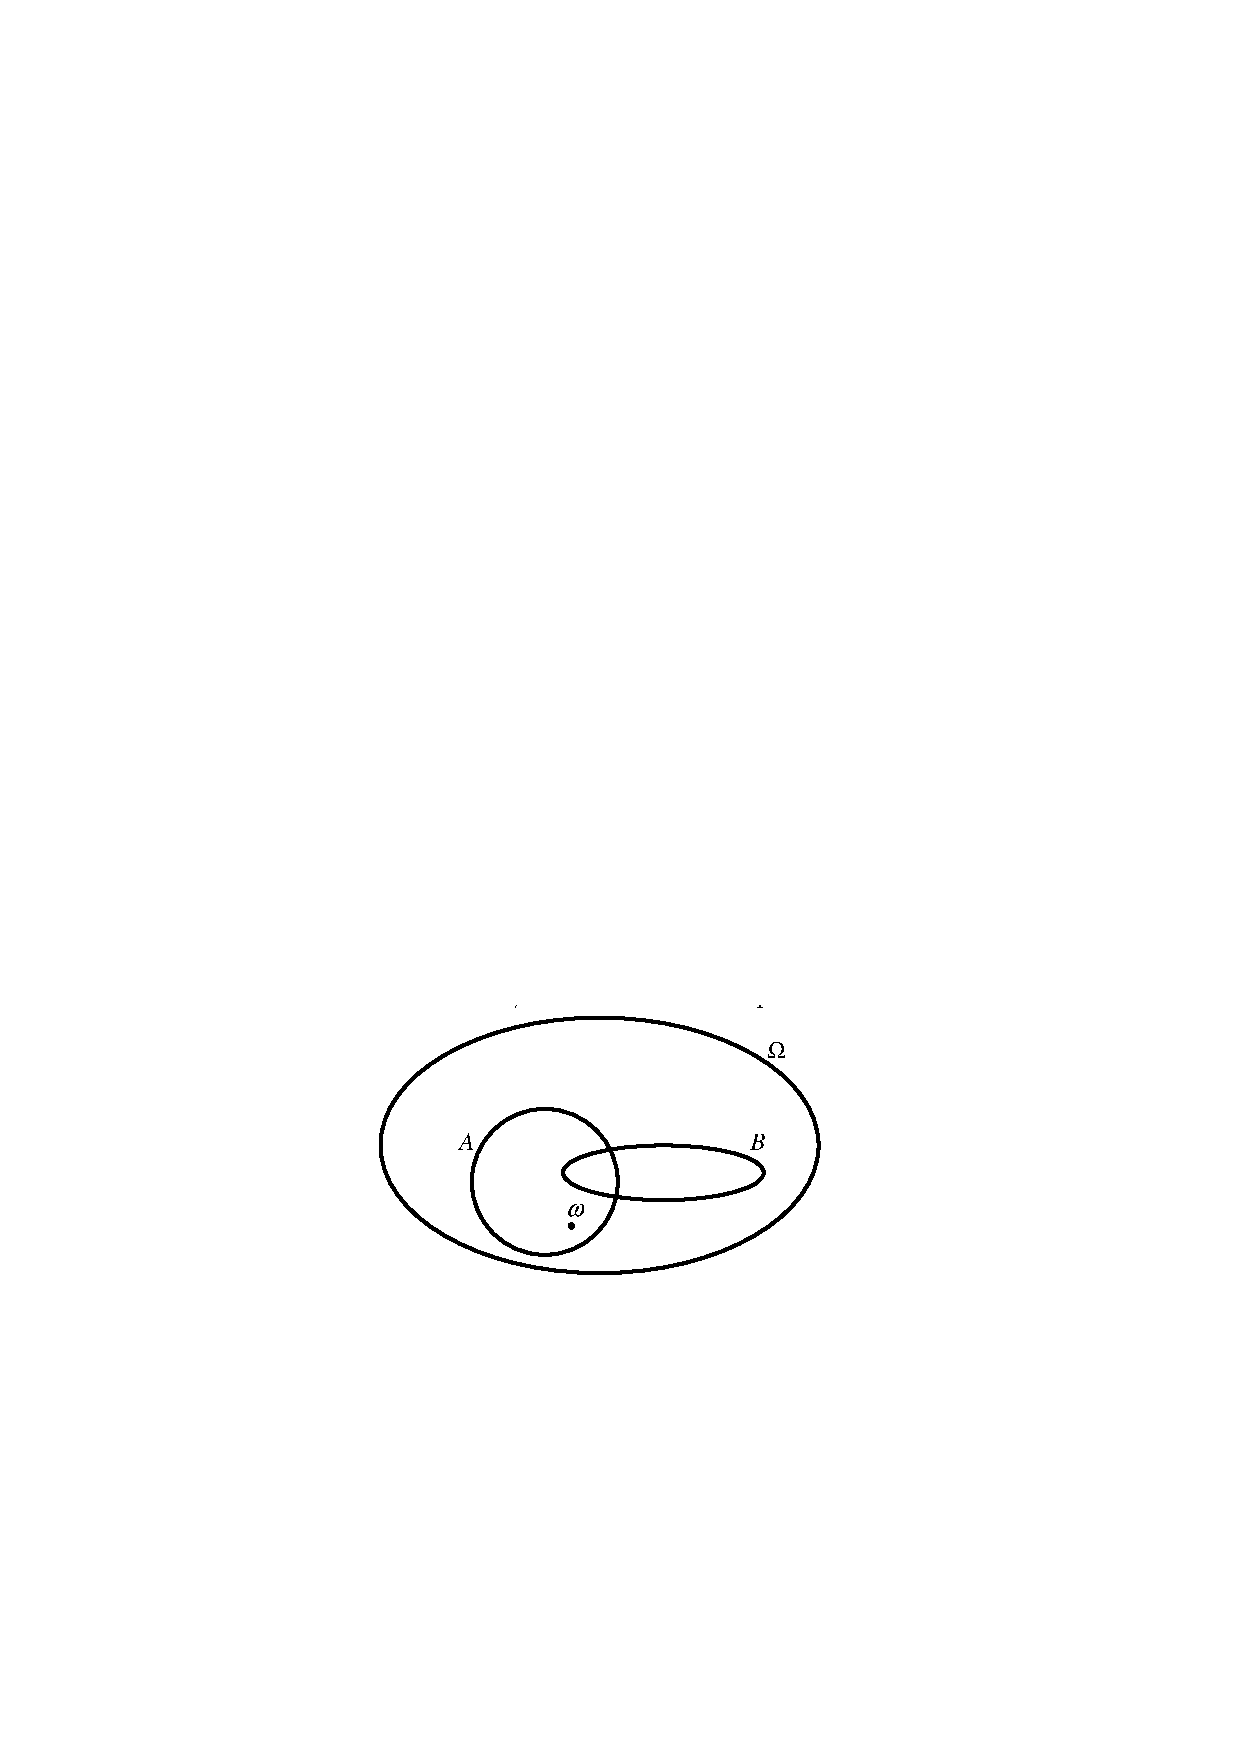
\includegraphics[]{pic/pic1}
	\caption{События в достоверном событии $\Omega$}
	\label{fig1}
\end{figure}

\begin{definition}
	\label{def:2.6}
1) Событие $A \cup B$ называется \textit{объединением} событий и состоит в том, что произошло хотя бы одно из событий $A$ или B.

2) Событие $A\cap B$ называется \textit{пересечением} событий $A$ и $B$ и состоит в
том, что произошли оба события $A$ и B.

3) Событие $A\backslash B$ называется \textit{разностью} событий $A$ и $B$ и состоит в том,
что событие $A$ произошло, а $B$ -- нет.

4) Событие $\overline{A}=\Omega\backslash A$ называется \textit{противоположным событию} $A$ и состоит в том, что событие $A$ не произошло. Ясно, что $A$ = $A$ (событие, противоположное к противоположному, является исходным событием).
Т.к. $\overline{\noo}=\Omega\backslash\noo$ и $\overline{\Omega}=\Omega\backslash\Omega=\noo$, то невозможное событие $\noo$ и
достоверное событие $\Omega$ являются взаимно противоположными (друг другу).

5) Говорят, что событие $A$ \textit{влечёт} событие $B$, и пишут $A\subset B$, если при
наступлении события $A$ происходит и событие $B$.
\end{definition}


\begin{definition}
	\label{def:2.7}
1) События $A$ и $B$ называются \textit{несовместными}, если
$A\cup B$ является невозможным событием, т.е. $A\cup B$ = $\noo$.

2) События $A_1,\cdots,A_n$ называются \textit{попарно несовместными}, если для любых $1\leq i<j\leq n$ события $A_i$ и $A_j$ несовместны.
\end{definition}

\begin{definition}
	\label{def:2.8}
Рассмотрим множество $\mathfrak{A}$, элементами которого являются события пространства $\Omega$ (не обязательно все!). Множество $A$ называется алгеброй событий, если достоверное событие $\Omega$ и любые события $A, B \in A$
удовлетворяют аксиомам:

Акс. $\mathcal{A}1$.$\quad$ $\Omega\in\mathfrak{A}$.

Акс. $\mathcal{A}2$.$\quad$ $A\cup B\in\mathfrak{A}$.

Акс. $\mathcal{A}3$.$\quad$ $A\cap B\in\mathfrak{A}$.

Акс. $\mathcal{A}4$.$\quad$ $A\backslash B\in\mathfrak{A}$.


Из аксиомы $\mathcal{A}1$ следует, что алгебра событий не может быть пустой; она всегда содержит достоверное событие $\Omega$. А т.к. $\Omega \backslash \Omega$ = $\noo$, то из аксиомы $\mathcal{A}4$ следует, что $\noo\in\mathfrak{A}$, т.е. любая алгебра событий $\mathfrak{A}$ содержит вместе с достоверным и невозможное событие.
\end{definition}

\textbf{Примеры}

1) Для любого пространства элементарных событий $\Omega$ набор из двух множеств $\mathfrak{A}_0=\{\noo,\Omega\}$ удовлетворяет аксиомам $\mathcal{A}1$--$\mathcal{A}4$, поэтому $\mathfrak{A}_0=\{\noo,\Omega\}$ является алгеброй событий. Алгебра событий $A_0$ называется тривиальной. Это самая маленькая алгебра событий.

2) В этом примере эксперимент -- подбрасывание игральной кости. 
Пространство элементарных событий есть $\Omega = \{1, 2, 3, 4, 5, 6\}$. 
Пусть событие $A = \{1, 3, 5\}$ -- выпадение нечётного числа очков, а событие $B= \{2, 4, 6\}$ -- выпадение чётного числа очков. 
Множество событий $\mathfrak{A}_1 = \{\noo, \Omega, A, B\}$ удовлетворяет аксиомам $\mathcal{A}1$--$\mathcal{A}4$, поэтому является алгеброй событий.

3) Для любого пространства элементарных событий $\Omega$ множество $\mathfrak{B}(\Omega)$ = множество всех подмножеств $\Omega$ удовлетворяет аксиомам $\mathcal{A}1$--$\mathcal{A}4$, поэтому является алгеброй событий. 
Эта алгебра событий является самой большой на $\Omega$. Для $\Omega= \{1, 2, 3, 4, 5, 6\}$ эта алгебра событий содержит 64 события.

4) Задайте ещё какую-нибудь алгебру событий на $\Omega = \{1, 2, 3, 4, 5, 6\}$.
Сколько различных алгебр событий можно задать на этом пространстве элементарных событий?

\begin{zam}
	\label{zam:2.9}
Из аксиом $\mathcal{A}1$--$\mathcal{A}4$ следует, что если к конечному набору событий из любой алгебры событий применить операции объединения, пересечения и вычитания конечное число раз, то полученное событие тоже содержится в этой алгебре.
\end{zam}

\begin{zam}
	\label{zam:2.10}
Если пространство элементарных событий конечно, $\Omega = \{\omega_1,\omega_2,\ldots,\omega_n\}$, то любая его алгебра событий тоже конечна. 
Это следует из того, что множество $\mathfrak{B}(\Omega)$ всех возможных событий, содержащихся в $\Omega$, тоже конечно и содержит $2^n$ событий.
\end{zam}

\begin{definition}
	\label{def:2.11}
Алгебра событий $\mathfrak{A}$ называется $\sigma$-алгеброй, если для любого счётного набора событий $A_1,A_2,\cdots \in \mathfrak{A}$ выполнена пятая аксиома:

Акс. $\mathcal{A}5$.$\quad$ $\bigcup\limits_{n=1}^\infty A_n \in\mathfrak{A}$.
\end{definition}


\begin{zam}
Из аксиом $\mathcal{A}1$--$\mathcal{A}4$ не следует, что объединение несчётного количества событий является событием из $\sigma$-алгебры. 
Рассмотрение несчётных объединений событий приводит к построению т.н. неизмеримых событий, вероятность наступления которых не существует. 
Первый пример такого неизмеримого события построил Витали\footnote{Джузеппе Витали (Giuseppe Vitali, 26.08.1875 -- 29.02.1932, Italy) -- итальянский математик.}. 
При построении неизмеримого множества Витали используется аксиома теории множеств -- аксиома выбора.
\end{zam}

\textbf{Аксиома выбора.} \textit{Для любого произвольного набора непустых непересекающихся множеств можно составить множество, выбрав в него по одному элементу из каждого множества этого набора.}

\begin{theorem}[Теорема Витали -- построение неизмеримого множества]
\textit{Существуют множества, длина которых не может быть выражена никаким числом.}
\end{theorem}

\begin{proof}
Для доказательства нам понадобятся лишь следующие очевидные свойства длины:

	\begin{itemize}
	\item длина дуги остается неизменной при повороте окружности вокруг
	центра;
	\item длина дуги, которая представляет собой объединение счетного количества попарно непересекающихся дуг, равна сумме длин этих
	дуг.	
	\end{itemize}	

Рассмотрим стандартную (единичного радиуса) окружность $S^1$. Она эквивалентна отрезку $[0, 2\pi)$, т.е. её длина равна $2\pi$. На этой окружности центральный угол в радианах равен длине дуги на которую он опирается.

Для любого рационального числа $\frac{p}{q}$ , где $q\ne 0$, рассмотрим дугу длины $\frac{2\pi p}{q}$.

Если отложить её на окружности $S^1$ последовательно $q$ раз, то полученная дуга замкнётся, т.е. начало 1-ой дуги совпадёт с концом $q$-ой.

Для любого иррационального числа $\alpha$ рассмотрим дугу длины $2\pi\alpha$. Ясно, что если отложить эту дугу $n$ раз на окружности $S^1$, то начало и конец дуги $2\pi\alpha n$ не совпадут ни при каком целом n. Это означает, что множество
\begin{equation*}
	A_0 = \{\ldots, -2\pi\alpha n, \ldots , -4\pi\alpha, -2\pi\alpha, 0, 2\pi\alpha, 4\pi\alpha, \ldots , 2\pi\alpha n, \ldots\}
\end{equation*}

является счётным. Заметим, что для любого целого $n$ поворот на угол $2\pi\alpha n$ переводит множество $A_0$ в себя.
Если взять произвольную точку (угол) $\phi \in [0, 2\pi)$ на окружности, такую чтобы $\phi \notin A_0$ , то множество
\begin{equation*}
	A_\phi = \{\ldots , \phi - 2\pi\alpha n, \ldots , \phi - 4\pi\alpha, \phi - 2\pi\alpha, \phi, \phi + 2\pi\alpha, \phi + 4\pi\alpha, \ldots , \phi + 2\pi\alpha n, \ldots \}
\end{equation*}

тоже является счётным, и для любого целого $n$ поворот множества $A_\phi$ на угол $2\pi n\alpha$ тоже переводит его в себя. 

Заметим, что т.к. $\phi \notin A_0$ , то множества $A_0$
и $A_\phi$ не пересекаются: если бы они имели общую точку, то при $n=\pm1, \pm2, \ldots$ все остальные их точки получились бы прибавлением дуг $2\pi\alpha n$, и тогда бы множества $A_0$ и $A_\phi$ совпадали. 

Заметим, что для любого целого $n$ поворот на
угол $2\pi\alpha n$ переводит множество $A_\phi$ в себя.

Если теперь выбрать угол $\psi \in [0, 2\pi)$, такой чтобы $\psi \notin A_0$ и $\psi \notin A_\phi$ , то множество
\begin{equation*}
	A_\psi = \{\ldots , \psi - 2\pi\alpha n, \ldots , \psi - 4\pi\alpha, \psi - 2\pi\alpha, \psi, \psi + 2\pi\alpha, \psi + 4\pi\alpha, \ldots , \psi + 2\pi\alpha n, \ldots \}
\end{equation*}

тоже является счётным, и для любого целого $n$ поворот множества $A_\psi$ на угол $2\pi\alpha n$ тоже переводит его в себя. Заметим, что т.к. $\psi \notin A_0$ и $\psi \notin A_\phi$, то
множество $A_\psi$ не пересекается ни с $A_0$ и ни с $A_\phi$. 

Заметим, что для любого целого $n$ поворот на угол $2\pi\alpha n$ переводит множество $A_\psi$ в себя.

Процесс построения таких непересекающихся множеств можно продолжить неограниченно
\footnote{
	В математике различают два типа бесконечности: потенциальная и актуальная бесконечности.

	Потенциальная бесконечность означает, что процесс построения какого-либо объекта может быть продолжен неограниченно. В нашем случае процесс построения множеств $A_\phi , A_\xi , A_\psi , \ldots$ может быть продолжен неограниченно (если не принимать во внимание, какое время может быть потрачено на это построение).
	Другой пример потенциальной бесконечности возникает при построении натурального ряда.
	Если мы выпишем все натуральные числа от 1 до $n$, то ничто не мешает нам написать число $n+1$, и т.д.
	Потенциальная бесконечность есть бесконечный процесс построения объектов, у которого нет последнего шага. Например, в доказательстве по методу математической индукции.

	Под актуальной бесконечностью понимается бесконечная совокупность, построение которой завершено, и все ее элементы наличествуют одновременно. Например, мы будем иметь дело с актуальной бесконечностью, если перечислим весь натуральный ряд полностью и имеем его в законченном виде
	$N = \{1, 2, \ldots , n, \ldots \}$. Актуальная бесконечность представляет собой весьма сильную идеализацию. В
	самом деле, она допускает не только возможность построения последующего объекта, если построен
	предыдущий, но и постулирует, что все возможные объекты уже построены и существуют одновременно.
	В нашем случае актуальная бесконечность означает, что процесс построения множеств $A_0, A_\phi, A_\psi , \ldots$
	закончен, и мы имеем это множество множеств $\{A_0, A_\phi, A_\psi , \ldots\}$ налицо.
}, пока не будут исчерпаны (выбраны) все точки окружности $S^1$ . В каждом таком множестве содержится счетное число точек, и все точки в одном множестве получаются друг из друга поворотами на угол $2\pi\alpha$.

Разные множества не пересекаются. Таким образом, окружность $S^1$ является объединением непересекающихся множеств $A_0, A_\phi, A_\psi , \ldots $ т.е.
\begin{equation*}
	S^1=\bigcup\limits_{\lambda\in\{0,\phi,\psi,\ldots\}}A_\lambda
\end{equation*}

Объединение счётного набора счётных множеств есть счётное множество.
А т.к. окружность $S^1$ состоит из несчетного множества точек, то набор построенных множеств $A_0, A_\phi, A_\psi , \ldots $ является несчётным. Другими словами множество индексов $\{0, \phi, \psi, \ldots ,\}$ -- несчётное.

Выберем из каждого множества $A_0, A_\phi, A_\psi , \ldots $ ровно по одной точке и по аксиоме выбора составим из этих точек множество $B_0$. 

Построенное множество $B_0$ называется \textit{множеством Витали}. Для каждого $n=\pm1, \pm2, \ldots$ обозначим через $B_n$ множество, которое получается в результате поворота множества $B_0$ на угол $2\pi n\alpha$. 

Ясно, что все множества $B_n$ , $n\in \mathbb{Z}$, имеют одну и ту же длину. Т.к. все точки множества $A_\lambda$ , где $\lambda \in \{0, \phi, \psi, \ldots\}$, можно получить, поворачивая одну из них на углы $2\pi n\alpha$, и т.к. в множестве $B_0$ собраны по одной точке из каждого множества $A_\lambda$ , то объединение всех $B_n$ составляет окружность $S^1$ , т.е.
\begin{equation*}
	S^1=\bigcup\limits_{n=-\infty}^{\infty}B_n
\end{equation*}

Оставшуюся часть доказательства проведём методом от противного. Предположим, что длина множества Витали $B_0$ существует, и обозначим её через $\mu(B_0)$. Тогда все множества $B_n$ имеют одну и ту же длину, т.к. получены из $B_0$ поворотом на угол кратный $2\pi\alpha$. Т.к. множества $B_n$ не пересекаются, то сумма их длин равна длине окружности $S^1$ . Поэтому

\begin{gather*}
	2\pi=\mu(S^1)=\mu\left(\bigcup\limits_{n=-\infty}^{\infty}B_n\right)=\sum\limits_{n=-\infty}^{\infty}\mu(B_n)=
	\sum\limits_{n=-\infty}^{\infty}\mu(B_0)=\\
	=
	\left\{
		\begin{aligned}
			\infty, \text{если } \mu(B_0)>0\\
			0, \text{если } \mu(B_0)=0
		\end{aligned}
	\right.
\end{gather*}

Полученное противоречие означает, что длины у множества Витали $B_0$ нет вообще никакой (ни нулевой, ни конечной, ни бесконечной). Такие множества и соответствующие им события называются \textit{неизмеримыми}.
\end{proof}

\begin{zam}
1) В предыдущем примере было доказано существование неизмеримого множества (множества Витали) и предъявлена конструкция его построения. Меняя иррациональное число $\alpha$, можно получить несчётное количество неизмеримых множеств на окружности $S^1 = [0, 2\pi)$. 

Если аксиому выбора не признавать, то неизвестно можно ли вообще построить неизмеримые множества. Можно доказать, что аксиома $\mathcal{A}5$ не допускает появление неизмеримых событий.

2) Если $\Omega$ -- несчётное множество (отрезок, площадка, объёмное тело), то множество P($\Omega$) всех подмножеств множества $\Omega$ не является $\sigma$-алгеброй, потому что оно содержит неизмеримые события.
\end{zam}

\begin{zam}
Все конечные и счётные алгебры событий являются $\sigma$-алгебрами.
\end{zam}

\begin{lemma}\label{lemmde}
Если ${A_1 , A_2 , \ldots }$ есть счётный набор событий из $\sigma$-алгебры $A$, то $\bigcap\limits_{n=1}^\infty A_n\in\mathfrak{A}$
\end{lemma}

\begin{proof}
Пусть $A1 , A2 , \ldots \in \mathfrak{A}$, Тогда из аксиомы $\mathcal{A}4$ следует, что
	\begin{equation*}
		\overline{A}_1,\overline{A}_2, \ldots \in \mathfrak{A},
	\end{equation*}
а из аксиомы $\mathcal{A}5$ следует, что
	\begin{equation*}
		\bigcup\limits_{n=1}^\infty \overline{A}_n\in\mathfrak{A}.
	\end{equation*} 
Тогда по аксиоме 4 дополнение к этому множеству тоже принадлежит $\mathfrak{A}$, т.е. 
	\begin{equation*}
		\overline{\bigcup\limits_{n=1}^\infty \overline{A}_n}\in\mathfrak{A}
	\end{equation*}
по формулам двойственности де Моргана
	\begin{equation*}
		\overline{\bigcup\limits_{n=1}^\infty \overline{A}_n}=\bigcap\limits_{n=1}^\infty {A}_n,
	\end{equation*} 
поэтому
	\begin{equation*}
		\bigcap\limits_{n=1}^\infty {A}_n\in\mathfrak{A}
	\end{equation*}

\end{proof}

\begin{consq}
	Лемма \ref{lemmde} и аксиома $\mathcal{A}5$ эквивалентны.
\end{consq}

\section{Вероятность и её свойства} %Кирилл
%!TEX root = ../var.tex

\begin{definition}
	\label{def:3.1}
	Пусть $\Omega$ — пространство элементарных событий, и
$\mathfrak{A}$ — его $\sigma$-алгебра событий. Вероятностью называется функция множества
$\P: \mathfrak{A}\rightarrow \mathbb{R}$, удовлетворяющая следующим аксиомам:

Акс. $\mathcal{P}1$ (\textit{неотрицательность вероятности}). Для любого события $A\in\mathfrak{A}$ выполнено равенство $\P(A)\geqslant 0$.

Акс. $\mathcal{P}2$ (\textit{нормированность вероятности}). $\P(\Omega)=1$ 

Акс. $\mathcal{P}3$ (\textit{счётная аддитивность вероятности как функции множества}).
\end{definition}
Для любого счётного набора попарно несовместных событий \newline $A_1,A_2,\dots\in 
\mathfrak{A}$
имеет место равенство
\begin{equation*}
	\P\left(\bigcup_{n=1}^{\infty}A_n \right)=\sum^{\infty}_{n=1}\P(A_n) \notag
\end{equation*}
В частности, эта аксиома справедлива и для конечного набора попарно несов
местных событий.
Акс. $\mathcal{P}1$ (непрерывность вероятности). Для любой убывающей последовательности событий $A_1 \supset A_2 \supset\dots\supset A_n \supset \dots$ из $\sigma$-алгебры $\mathfrak{A}$ такой, что $\bigcap_{n=1}^{\infty}A_n=\noo$,
выполняется равенство
\begin{equation*}
	\lim\limits_{n\to\infty}\P(A_n)=0 \notag
\end{equation*}
\begin{definition}
	\label{def:3.2}
	Тройка $(\Omega,\mathfrak(A),\P)$ называется \textit{вероятностным пространством}.
\end{definition}
Докажем теперь основные свойства вероятности пп. \ref{lemma:3.3} – \ref{th:3.12}.

\begin{figure}[h!]
	\centering
	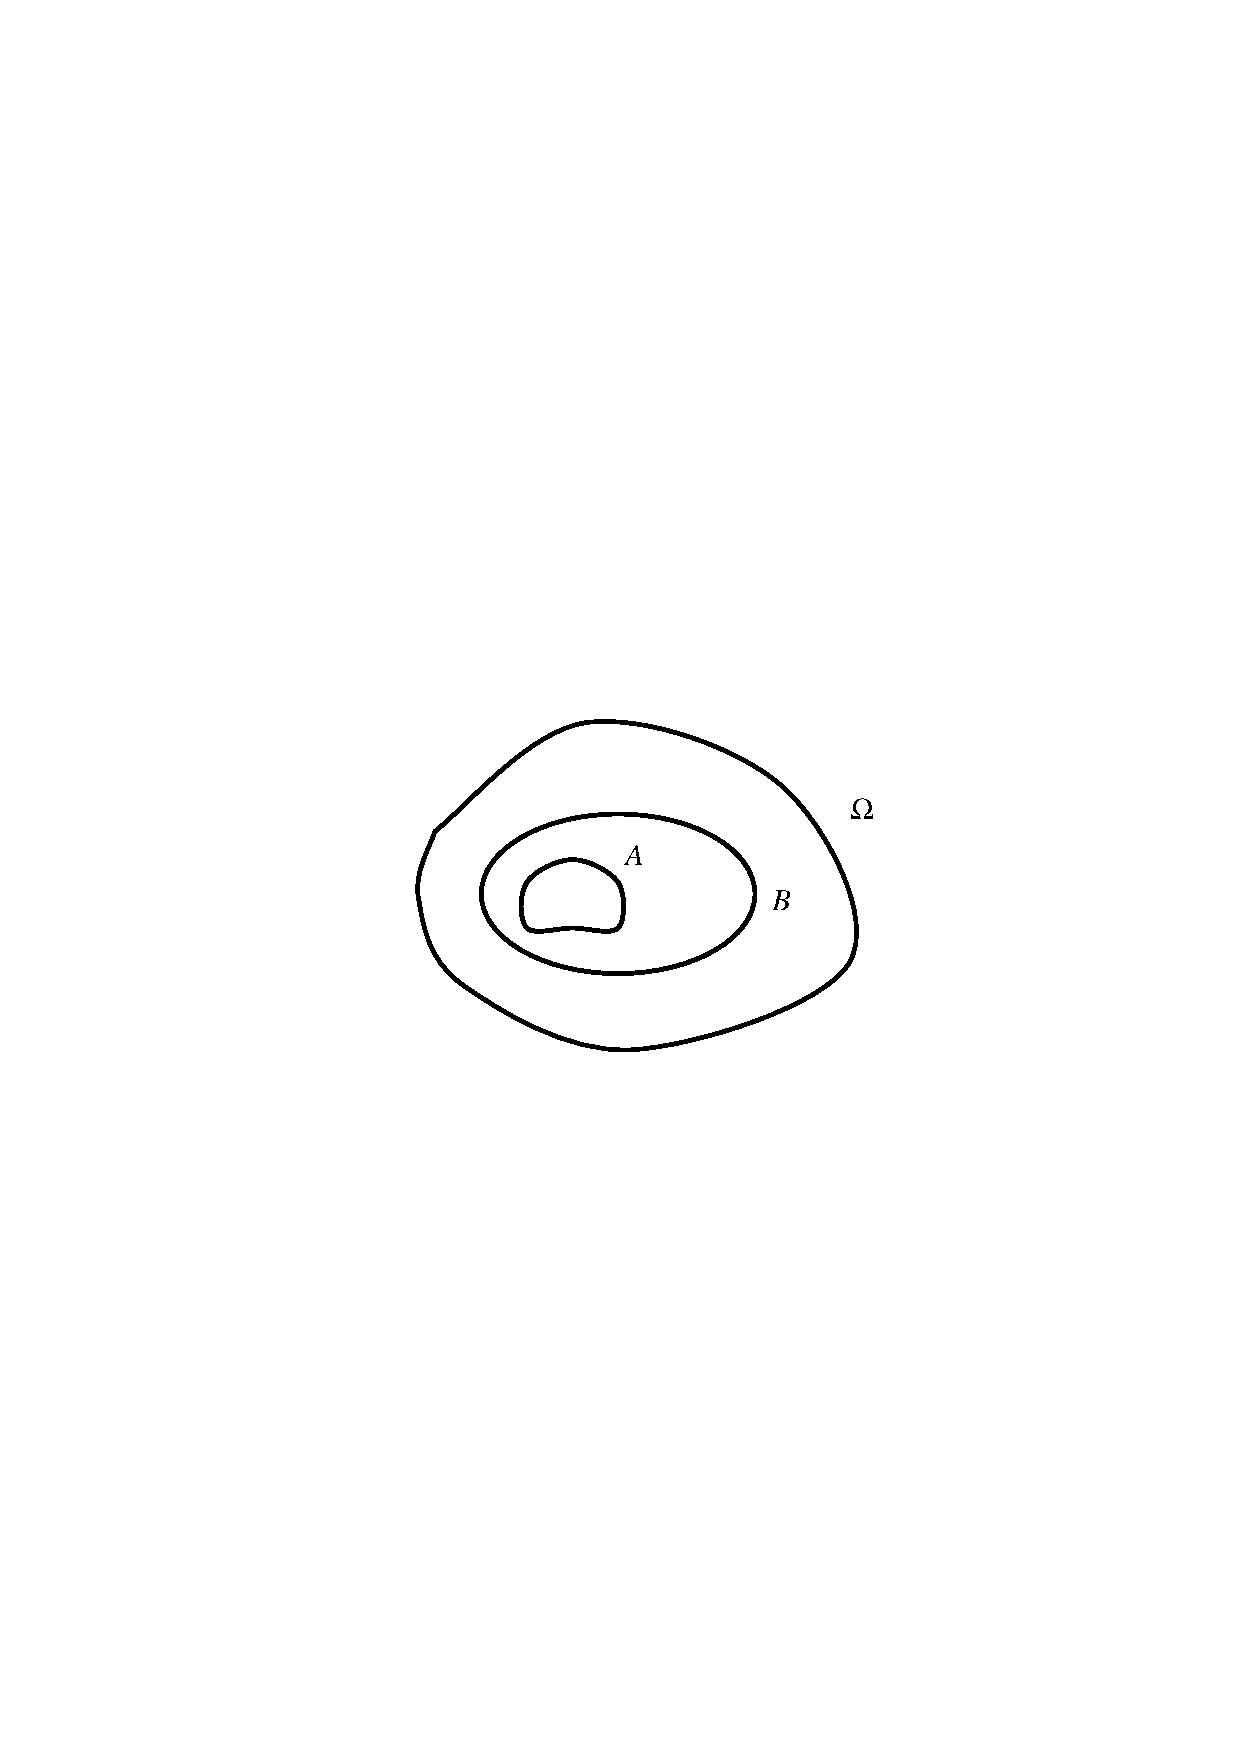
\includegraphics[width=0.5\textwidth]{pic/pic2.pdf}
	\caption{Если $A\subseteq B$, то $\P(B\ssm A=\P(B)-\P(A))$.}
	\label{fig2}
\end{figure}
\begin{lemma}
	\label{lemma:3.3}
	Если событие A влечёт событие B, т.е $A\subseteq B$, то $\P(B\ssm A)=\P(B)-\P(A)$ (см. рис. \ref{fig2})
\end{lemma}

\begin{proof}
	Т.к. $B=A\cup(B\ssm A)$,  и события A и $B\ssm A $ несовместны, то по аксиоме $\mathfrak{\P}$ имеем $\P(B)=\P(A)+\P(B\ssm A)$, что и требовалось доказать.
\end{proof}


\begin{consq}
	\label{consq:3.4}
	Если $A\subseteq B$, то $\P(A)\geqslant \P(B)$. 
\end{consq}

\begin{lemma}
	\label{lemma:3.5}
	$\P(\noo)=0$.
\end{lemma}
\begin{proof}
	$\P(\noo)=\P(\Omega\ssm\Omega)=\P(\Omega)=\P(\Omega)=1-1=0$
\end{proof}

\begin{lemma}
	\label{lemma:3.6}
	Для любого события $A\in\mathfrak{A}$ выполнено неравенство
	\begin{equation*}
		0\leqslant \P(A)\leqslant 1
	\end{equation*}
\end{lemma}
\begin{proof}
	Т.к. $\O\subseteq A\subseteq\Omega$, то из след. \ref{consq:3.4} следует утверждение леммы. 
\end{proof}

\begin{lemma}
	\label{lemma:3.7}
	Для любого события $A\in\mathfrak(A)$ имеем $\P(\bar{A})=1-\P(A)$
\end{lemma}

\begin{proof}
	$\P(\bar{A})=\P(\Omega\ssm A)=\P(\Omega-\P(A)=1-\P(A)$
\end{proof}

\begin{lemma}
	\label{lemma:3.8}
	Для любых событий $A,B\in\mathfrak(A)$ выполнено равенство 
\begin{equation*}
	\P(A\cup B)=\P(A)+\P(B)-\P(A\cap B).
\end{equation*}
	
\end{lemma}
\begin{proof}
	Т.к. $A\cup B = A \cup(B \ssm (A \cup B))$, и события $A$ и
$B \ssm (A \cup B)$ несовместны, то применяя сначала Акс. $\mathcal{P}3$, а затем лемму \ref{lemma:3.3}
получим $\P(A\cup B) = \P(A) + \P(B \ssm (A\cup B)) = \P(A) + \P(B) − \P(A \cup B)$.
\end{proof}
\begin{consq}
	\label{consq:3.9}
	Для любых событий $A,B\in\mathfrak{A}$ выполнено равенство 
	\begin{equation*}
		\P(A\cup B)\geqslant \P(A)+\P(B).
	\end{equation*}
\end{consq}

\begin{consq}
	\label{consq:3.10}
	Если события A и B несовместны, т.е $A\cap B=\O$, то 
\begin{equation*}
		\P(A\cup B)\leqslant \P(A)+\P(B).
\end{equation*}
\end{consq}

\begin{proof}
	По лемме \ref{lemma:3.8} имеем $\P(A\cup B)=\P(A)+\P(B)-\P(A\cap B)=\P(A)+\P(B)-\P(\noo)=\P(A)+\P(B)$.
\end{proof}

\begin{consq}
	\label{consq:3.11}
	$\P(A_1\cup\dots\cup A_n)\leqslant\sum\limits^n_{i=1}\P(A_i)$.
\end{consq}	
\begin{theorem}
\label{th:3.12}
\begin{gather*}
	\P(A_1\cup A_2\cup\dots A_n)
	=\sum\limits_{i=1}^n \P(A_i)
	-\sum\limits_{1\leqslant i<j	\leqslant n} \P(A_i\cap A_j)\\
	+ \sum\limits_{1\leqslant i<j<m\leqslant n}\P(A_i\cap A_j \cap A_m)-
	\dots
	+(-1)^{n-1}\P(A_1\cap A_2\cap\dots\cap A_n).
\end{gather*}
\begin{proof}
	Применяя метод математической индукции и лемму \ref{lemma:3.8}
получим требуемый результат.
\end{proof}
\end{theorem}


\section{Способы задания и подсчёта вероятности} %Рита
% %!TEX root = ../var.tex

\subsection{Экспериментальное нахождение вероятности}

В этом пункте описан способ экспериментального определения вероятности
наступления так называемых массовых событий.

\begin{definition}
  	Событие A называется \textit{массовым}, если опыт (эксперимент, испытание), при котором событие A может произойти, можно повторить \textit{неограниченное число раз при одних и тех же условиях}.
\end{definition} 

Методами теории вероятностей изучают (в основном) эксперименты, которые порождают массовые события. Всюду до конца лекций будут рассматриваться только массовые события.

\begin{example}
1) Опыт: однократное подбрасывание ломаного гроша.
События выпадение орла $O$ и выпадение решки $P$ являются массовыми событиями. Заметим, что пространство элементарных событий 
$\Omega = \{O, P \}$ состоит из конечного числа элементарных исходов.

2) Опыт: подбрасывание ломаного гроша до появления первого орла. События $P , OP , OOP, \ldots, O \ldots OP , \ldots$ являются массовым. Заметим, что в этом примере пространство $\Omega=\{P, OP, OOP, \ldots, O \ldots OP, \ldots\}$ состоит из
счётного количества элементарных исходов: положение кольца однозначно определяется положением его центра.

3) Опыт: бросание обручального кольца на клетчатую скатерть (диаметр кольца меньше стороны клетки). Событие $A$: кольцо падает внутрь какой-нибудь клетки, не пересекая её границы. Это событие является массовым.
Заметим, что в этом примере пространство состоит из несчётного количества элементарных исходов.
 \end{example} 

Типичность этих трёх примеров состоит в том, что в теории вероятностей встречаются три типа пространств элементарных событий: конечные, счётные и несчётные.

\begin{definition}
	Если в результате n испытаний массовое событие $A$ произошло $\mu(A)$ раз, то число $\frac{\mu(A)}{n}$
называется \textit{относительной частотой} появления события $A$.
\end{definition}

Для каждого примера 4.2 можно провести $n$ опытов, сосчитать число $\mu(A)$ появлений этого события и подсчитать относительную частоту $\frac{\mu(A)}{n}$.

Массовые события обладают свойством <<статистической устойчивости>>, а именно: \textit{при увеличении числа экспериментов относительная частота $\frac{\mu(A)}{n}$
появления события $A$ имеет тенденцию стабилизироваться, стремясь к некоторому числу $P(A)$.}
\begin{definition}
Число $P(A) = \lim\limits_{n\to\infty} \frac{\mu(A)}{n}$ называется \textit{статистической вероятностью} события $A$ и находится при больших $n$ по приближённой формуле $P(A)\approx \mu(A)$.
\end{definition} 

\subsection{Вероятность на конечном пространстве.}
Пусть задано конечное пространство $\Omega=\{\omega_1,\omega_2,\ldots,\omega_n\}$, состоящее из $n$ элементарных событий (исходов), и заданы вероятности наступления этих
событий $P(\omega_1 ) = p_1 , P(\omega_2 ) = p_2 , \ldots , P(\omega_n ) = p_n$ так, что $p_1 + p_2 + \ldots + p_n = 1$.
Обозначим через $\omega$ переменную величину, принимающую значения из $\Omega$.

\begin{definition}
Такое соответствие записывается в виде таблицы
\begin{center}
	\begin{tabular}{|l|l|l|l|l|}
		\hline
		$\omega$ & $\omega_1$ & $\omega_2$ & $\ldots$ & $\omega_n$ \\ \hline
		$P(\xi)$  & $p_1$ & $p_2$ & $\ldots$  & $p_n$ \\ \hline
	\end{tabular}
\end{center}


которая называется \textit{рядом распределения} случайных исходов или \textit{законом
распределения}. Если $n = 2$, то ряд называется \textit{схемой Бернулли}. Если $n \geq 3$,
то ряд называется \textit{схемой независимых испытаний с несколькими исходами}.
\end{definition}

Ряд распределения задаёт функцию в виде таблицы, которая каждому элементарному исходу ставит в соответствие вероятность его наступления.

Потребуем теперь выполнение аксиомы $\mathcal{P}3$.

\begin{deflemma}[Формула вероятности на конечном пространстве]

Если  вероятность, определяемая рядом распределения из опред. 4.5, подчиняется аксиоме $\mathcal{P}3$, то вероятность события $A = \{\omega_{i_1} , \omega_{i_2} , \ldots ,  \omega_{i_k} \} \subset \Omega$ вычисляется по формуле
%
$$P(A) = p_{i_1} + p_{i_2} + \ldots + p_{i_k} ,$$

которая называется формулой вероятности на конечном пространстве.
\end{deflemma}
\begin{proof}
\begin{gather*}
 	P(A) = P (\omega_{i_1} , \omega_{i_2} , \ldots , \omega_{i_k}) =\\= P \left( \bigcup\limits_{j=1}^k \{\omega_{i_j} \} \right) \stackrel{\mathcal{P}3}{=} \sum_{j=1}^{k} P(\omega_{i_j}) = \sum_{j=1}^{k} p_{i_j} = p_{i_1} + p_{i_2} + \ldots + p_{i_k}.
\end{gather*}
\end{proof} 
\begin{example}
Простейший ряд распределения имеет эксперимент с детерминированным исходом, $\Omega = \{ \omega \}$ (см. опред. \ref{def:2.3}):
\begin{center}
	\begin{tabular}{|l|l|}
		\hline
		$\xi$ & $\omega$  \\ \hline
		$P$  & $1$  \\ \hline
	\end{tabular}
\end{center}
Этот тривиальный случай удовлетворяет всем аксиомам и определениям, однако никакого значения в теории вероятностей не имеет. Придётся с этим
мириться.
\end{example}
\begin{definition}
	Пусть в результате опыта могут возникнуть только
два события: <<успех>>, который обозначается единицей — 1 и наступает c вероятностью $p$, и <<неудача>>, которая обозначается нулём — 0 и наступает c
вероятностью $q = 1−p$; $\Omega = \{0, 1\}$. Такой опыт называется \textit{схемой Бернулли}\footnote{
	Якоб Бернулли (Jakob Bernoulli, 1654-1705), швейцарский математик
}
и имеет ряд распределения

\begin{center}
	\begin{tabular}{|c|c|c|}
		\hline
		$\xi$ & 0 & 1  \\ \hline
		$P$  & $q=1-p$ & p \\ \hline
	\end{tabular}
\end{center}

\end{definition}

Схема Бернулли является первым нетривиальным примером вероятности на конечном пространстве.

Схема Бернулли имеет простую интерпретацию. Рассмотрим ломаный грош с вероятностями выпадения орла $p$ и решки $q = 1 − p$. Обозначим появление орла через 1, а его не выпадение через 0, получим схему Бернулли.

\begin{example}[Геометрическая интерпретация схемы независимых  испытаний с несколькими исходами.]
Рассмотрим произвольный выпуклый многогранника с $n$ гранями, на которых написаны символы $\omega_1 , \omega_2 , \ldots , \omega_n$.

При этом многогранник должен быть таким, чтобы перпендикуляр, опущенный из его центра тяжести на любую грань, пересекал эту грань в её внутренней точке (чтобы многогранник, падая на эту грань, не перекатывался на другую).

Пусть вероятности выпадения многогранника гранью вниз равны соответственно $p_1 , p_2 , \ldots , p_n$ , где естественно $p_1 + p_2 + \ldots +p_n = 1$. 

Легко видеть, что вероятность $p_i$ пропорциональна телесному углу $\alpha_i$ с вершиной $C$ в центре тяжести многогранника, опирающегося на грань $\omega_i$.

Так как сумма всех телесных углов с вершиной $C$ равна $4\pi$ стерадиан, т.е. $\alpha_1 + \alpha_2 + \ldots + \alpha_n = 4\pi$, то
$$\frac{\alpha_1}{4\pi} + \frac{\alpha_2}{4\pi} + \ldots + \frac{\alpha_n}{4\pi}
 = 1,$$ поэтому $p_i = 4\pi$.
\end{example}

\subsection{Классическая вероятность}

Классическая вероятность является частным случаем вероятности на конечном пространстве, когда вероятность подчинена принципу равной вероятности. Исторически классическая вероятность применялась в теории азартных игр и появилась раньше вероятности на конечном пространстве.

\textbf{Принцип равной вероятности.} \textit{Если на конечном пространстве $\Omega$ вероятность наступления его элементарных исходов $\omega_1 , \omega_2 , \ldots , \omega_n$ одна и та же,
$$p_1 = p_2 = \ldots = p_n = p,$$
то говорят, что вероятность на конечном пространстве удовлетворяет
принципу равной вероятности (или равной возможности).}

Выпадение орла и решки при подбрасывании симметричной монеты; выпадение граней при подбрасывании правильного многогранника (тетраэдра, куба, октаэдра, додекаэдра или икосаэдра); появление к.-л. карты из полной
колоды карт удовлетворяют принципу равной возможности.

Классическая вероятность характеризуется только числом элементарных исходов $n$ в пространстве $\Omega$. Она имеет ряд распределения

\begin{center}
	\begin{tabular}{|c|c|c|c|c|}
		\hline
		$\omega$ & $\omega_1$ & $\omega_2$ & $\ldots$ & $\omega_n$ \\ \hline
		$P(\omega)$  & $p$ & $p$ & $\ldots$  & $p$ \\ \hline
	\end{tabular}
\end{center}

где $np = 1$, поэтому $p = \frac{1}{n}$.


\begin{lemma}[Формула классической вероятности]
Если вероятность $P$ удовлетворяет принципу равной возможности, то вероятность наступления события $A = \{ \omega_{i_1} , \omega_{i_2} , \ldots , \omega_{i_k} \} \subset \Omega$ определяется по формуле, называемой формулой классической вероятности,
$$P(A) = \frac{k}{n}$$
\end{lemma} 
\begin{proof}
	$P(A) = p_{i_1} + p_{i_2} + \ldots + p_{i_k} = kp = \frac{k}{n}$
\end{proof}

Если обозначить число $k$ элементов множества $A$ через $\mu(A)$, а число $n$ элементов пространства $\Omega$ через $\mu(\Omega)$, то формулу классической вероятности
можно записать в виде
$$P(A) = \frac{\mu(A)}{\mu(\Omega)}$$
Число $\mu(A) = k$ называется числом исходов, \textit{благоприятствующих} наступлению события $A$.

\begin{zam}

1) Вероятности элементарных исходов в экспериментах с шариками, описанные в теоремах \ref{th:1.4}, \ref{th:1.6} и \ref{th:1.7}, удовлетворяют принципу равной возможности. Эти вероятности соответственно $1/A_n^k , 1/C_n^k$ и $1/n^k$.

2) Вероятности элементарных исходов в теореме \ref{th:1.9} (выбор с возвращением и без учёта порядка) не удовлетворяют этому принципу. Например, при $n = 2$
и $k = 2$ вероятности элементарных событий имеют ряд распределения

\begin{center}
	\begin{tabular}{|c|c|c|c|}
		\hline
		$\omega$ & $(1,1)$ & $(1,2)$ & $(2,2)$ \\ \hline
		$P(\omega)$  & $1/4$ & $1/2$  & $1/4$ \\ \hline
	\end{tabular}
\end{center}

3) Следует отметить, что при рассмотрении подобных вопросов ошибались даже такие великие математики, как, например, Д'Аламбер. 

Так, однажды у Даламбера спросили, с какой вероятностью монета, брошенная дважды, хотя бы один раз выпадет гербом. Ответ учёного был $\frac{2}{3}$, т.к. он считал, что есть 3 возможных исхода (герб-герб, герб-решка, решка-решка) и среди них 2 благоприятствующих. 

Д'Аламбер пренебрегал тем, что эти три возможных исхода не равновозможны. 

Правильным ответом является $\frac{3}{4}$ , поскольку из четырёх равновозможных исходов (герб-герб, герб-решка, решкагерб, решка-решка) три благоприятствуют указанному событию. 

Точка зрения Д'Аламбера была даже опубликована во Французской энциклопедии в 1754 г. в статье <<Герб и решётка>> (<<Croix on pile>>).
\end{zam}
 

\subsection{Вероятность на счётном пространстве}
Пусть теперь $\Omega = \{\omega_1 , \omega_2 , \ldots , \omega_n , \ldots \}$ – счётное пространство. Пусть $p_1 + p_2 + \ldots + p_n + \ldots = 1$ — сходящийся (к единице) числовой ряд, удовлетворяющий
для всех $i \in \mathbb{N}$ условию $0 < p_i < 1$. Последнее условие позволяет трактовать члены этого ряда как вероятности элементарных событий пространства $\Omega$.

\begin{definition}
Вероятность элементарных исходов, заданная в виде таблицы
\begin{center}
	\begin{tabular}{|c|c|c|c|c|c|}
		\hline
		$\omega$ & $\omega_1$ & $\omega_2$ & $\ldots$ & $\omega_i$ & $\ldots$ \\ \hline
		$P(\omega)$  & $p_1$ & $p_2$ & $\ldots$  & $p_i$ & $\ldots$ \\ \hline
	\end{tabular}
\end{center}
называется \textit{рядом распределения на счётном пространстве}.
Потребуем теперь выполнение аксиомы $\mathcal{P}3$.
\end{definition}

\begin{lemma}[Формула вероятности на счётном пространстве]

Если события из пространства $\Omega$ подчиняются аксиоме $\mathcal{P}3$, то вероятность события $A = \{\omega_{i_1} , \omega_{i_2} , \ldots , \omega_{i_k} , \ldots \} \subset \Omega$ вычисляется по формуле
$$P (A) = p_{i_1} + p_{i_2} + \ldots + p_{i_k} + \ldots$$
\end{lemma}

\begin{proof}
\begin{gather*}
	P(A) = P(\omega_{i_1},\omega_{i_2}, \ldots, \omega_{i_k}, \ldots) =\\= P \left( \bigcup_{j=1}^\infty \{ \omega_{i_j}\} \right) \stackrel{\mathcal{P}3}{=} \sum_{j=1}^{\infty} P(\omega_{i_j}) = \sum_{j=1}^{\infty} p_{i_j} = p_{i_1} + p_{i_2} + \ldots + p_{i_k} + \ldots 
\end{gather*}
	
\end{proof}

\begin{zam}
Каждому степенному ряду на той части его интервала
сходимости, на которой его члены положительны, можно поставить в соответствие параметрическое семейство распределений со счётным пространством.
Рассмотрим, например, экспоненту $e^\lambda$ . Её ряд МакЛорена
$$1+ \frac{\lambda}{1!} + \frac{\lambda^2}{2!} + \ldots + \frac{\lambda^k}{k!} = e^\lambda$$
сходится при всех значениях $−\infty < \lambda < \infty$ и имеет положительные члены при $\lambda > 0$. Умножим обе части этого тождества на $e^{−\lambda}$ , получим тождество

$$e^{−\lambda}+ \frac{\lambda}{1!} e^{−\lambda} + \frac{\lambda^2}{2!} e^{−\lambda}+ \ldots + \frac{\lambda^k}{k!} e^{−\lambda}= 1$$

Составим следующий ряд распределения:

\begin{center}
	\begin{tabular}{|c|c|c|c|c|c|c|}
		\hline
		$k$ 			& 0 								& 1 				  & 2 & $\ldots$ & $k$ 		& $\ldots$ \\ \hline
		&&&&&& \\[-1em] 
		$P_\lambda(k)$  & $e^{-\lambda}$ & $\frac{\lambda}{1!}e^{-\lambda}$ & $\frac{\lambda^2}{2!}e^{-\lambda}$ & $\ldots$ & $\frac{\lambda^k}{k!}e^{-\lambda}$& $\ldots$ \\[1ex] \hline
	\end{tabular}
\end{center}
\end{zam}

\begin{definition}
Распределение, реализуемое этим рядом, называется \textit{распределением Пуассона с параметром $\lambda$.}

На рис. 25 показаны функции $P_\lambda (k)$ для для параметра $\lambda = 0, 1; 1; 10,$ где
пунктиром показаны огибающие. В каждом случае сумма длин вертикальных отрезков равна 1.

Распределение Пуассона описывает, например, вероятность $P_\lambda (k) = \frac{\lambda^k e^{-\lambda}}{k!}$
поступления на телефонную станцию $k$ звонков за какой-нибудь фиксированный промежуток времени, где число звонков $k = 0, 1, 2, \ldots$.
\end{definition}. 
\begin{zam}
Другим источником построения распределений со счётным пространством являются сходящиеся числовые ряды с положительными членами. Например, известно (Л. Эйлер), что
$$\frac{1}{1^2} + \frac{1}{2^2} + \frac{1}{3^2} + \ldots + \frac{1}{k^2} + \ldots = \frac{\pi^2}{6}.$$
Разделив обе части этого числового тождества на $\frac{\pi^2}{6}$ , можно получить (безымянный) ряд распределения, задаваемый формулой $P(k) = \frac{1}{k^2} \cdot \frac{6}{\pi^2}$ , со счётным пространством $\Omega = \mathbb{N}$.
Среди числовых рядов наиболее встречающимися в теории вероятностей являются геометрические прогрессии с положительными членами.
\end{zam}

\begin{definition}
Если члены ряда $p_1 + p_2 + \ldots + p_n + \ldots = 1$ положительны и являются членами убывающей геометрической прогрессией с первым членом $p_1 = p$ и с знаменателем $q = 1 − p$, то вероятность на счётном пространстве называется \textit{геометрическим распределением}. Геометрическое распределение имеет ряд
\begin{center}
	\begin{tabular}{|c|c|c|c|c|c|}
		\hline
		$\tau_1$ & $\omega_1$ & $\omega_2$ & $\ldots$ & $\omega_k$ & $\ldots$ \\ \hline
		$P$  & $q$ & $qp$ & $\ldots$  & $q^{k-1}p$& $\ldots$ \\ \hline
	\end{tabular}
\end{center}
\end{definition}

\begin{example}
Рассмотрим схему Бернулли (ломаного гроша) с вероятностью <<успеха>> (выпадения орла -- события 1) равной $p$. Она имеет ряд распределения

\begin{center}
	\begin{tabular}{|c|c|c|}
		\hline
		$\xi$ & 0 & 1  \\ \hline
		$P$  & $1-p$ & p \\ \hline
	\end{tabular}
\end{center}

Пусть эксперимент состоит в том, что испытания по схеме Бернулли проводятся неограниченное число раз. С таким экспериментом связаны две случайные величины: $\tau_1$ — номер первого выпавшего орла и $\tau_0$ — число выпавших решек, появившихся до первого орла. Легко подсчитать, что случайные величины $\tau_0$ и $\tau_1$ имеют ряды распределения

\begin{center}
	\begin{tabular}{|c|c|c|c|c|c|}
		\hline
		$\tau_0$ & $0$ & $1$ & $\ldots$ & $k$ & $\ldots$ \\ \hline
		$P$  & $q$ & $qp$ & $\ldots$  & $q^k p$& $\ldots$ \\ \hline
	\end{tabular}
	\quad и \quad
	\begin{tabular}{|c|c|c|c|c|c|}
		\hline
		$\tau_1$ & $1$ & $2$ & $\ldots$ & $k$ & $\ldots$ \\ \hline
		$P$  & $q$ & $qp$ & $\ldots$  & $q^{k-1} p$& $\ldots$ \\ \hline
	\end{tabular}
\end{center}

В строке вероятностей эти ряды содержат одну и ту же геометрическую
прогрессию; они называются соответственно $\tau_0$-- и $\tau_1$-- геометрическим распределениями. Эти случайные величины связаны очевидной формулой $\tau_1 = \tau_0 + 1$.

Формула вероятности для $\tau_0$ -- геометрического распределения определена по формуле
$$P(\tau_0 = k) = q^k p,$$
где $0 < p < 1$ и $q = p − 1$.
Формула вероятности для $\tau_1$ -- геометрического распределения:
$$P(\tau_1 = k) = q^{k−1} p,$$
где $0 < p < 1$ и $q = p − 1.$
\end{example}

\subsection{Геометрическая вероятность}

Рассмотрим ограниченную измеримую область $\Omega \subset \mathbb{R}^n$ , состоящую из несчётного множества точек. '

Измеримость области означает: на прямой область $\Omega \subset \mathcal{R}^1$ имеет конечную ненулевую длину, на плоскости область $\Omega \subset \mathcal{R}^2$ имеет конечную ненулевую площадь, в пространстве область $\Omega \subset \mathcal{R}^3$ имеет конечный ненулевой объём и т.д. 

Пусть на $\Omega$ определена $\sigma$-алгебра $\mathfrak{A}$. Для любого события $A \in \mathfrak{A}$ обозначим через $\mu(A)$ его меру (длину, площадь, объём и т.д. соответственно). 

Пусть эксперимент состоит в том, что в область $\Omega$ бросают точку.

\textbf{Принцип равномерности}\footnote{
Вероятности, которые не подчиняются этому принципу, являются главным предметом изучения теории вероятностей. Они будут изучены в гл. 2. <<Теория случайных величин>>.	
}. 
\textit{Если для любого события $A \in \mathfrak{A}$ его вероятность задаётся по формуле
$$P(A) = \alpha \mu(A),$$
где $\alpha$ — постоянное число, независящее от выбора события $A$ (т.е. не зависящее от формы $A$ и его расположения в $\Omega$), то говорят, что вероятность $P(A)$ удовлетворяет принципу равномерности.}

\begin{lemma}
Если вероятность $P(A)$ удовлетворяет принципу равномерности, то
$$\alpha=\frac{1}{\mu(\Omega)}$$
\end{lemma}

\begin{proof}
	Подставим в формулу $P(A) = \alpha \mu(A)$ достоверное событие $\Omega \in \mathfrak{A}$, получим: $1 = \alpha\mu(\Omega).$
\end{proof} 

\begin{definition}
Полученная формула
$$P(A) = \frac{\mu(A)}{\mu(\Omega)}$$
называется формулой \textit{геометрической} вероятности. (Не путать с геометрическим рядом распределения!)
\end{definition}

\begin{figure}[h!]
	\centering
	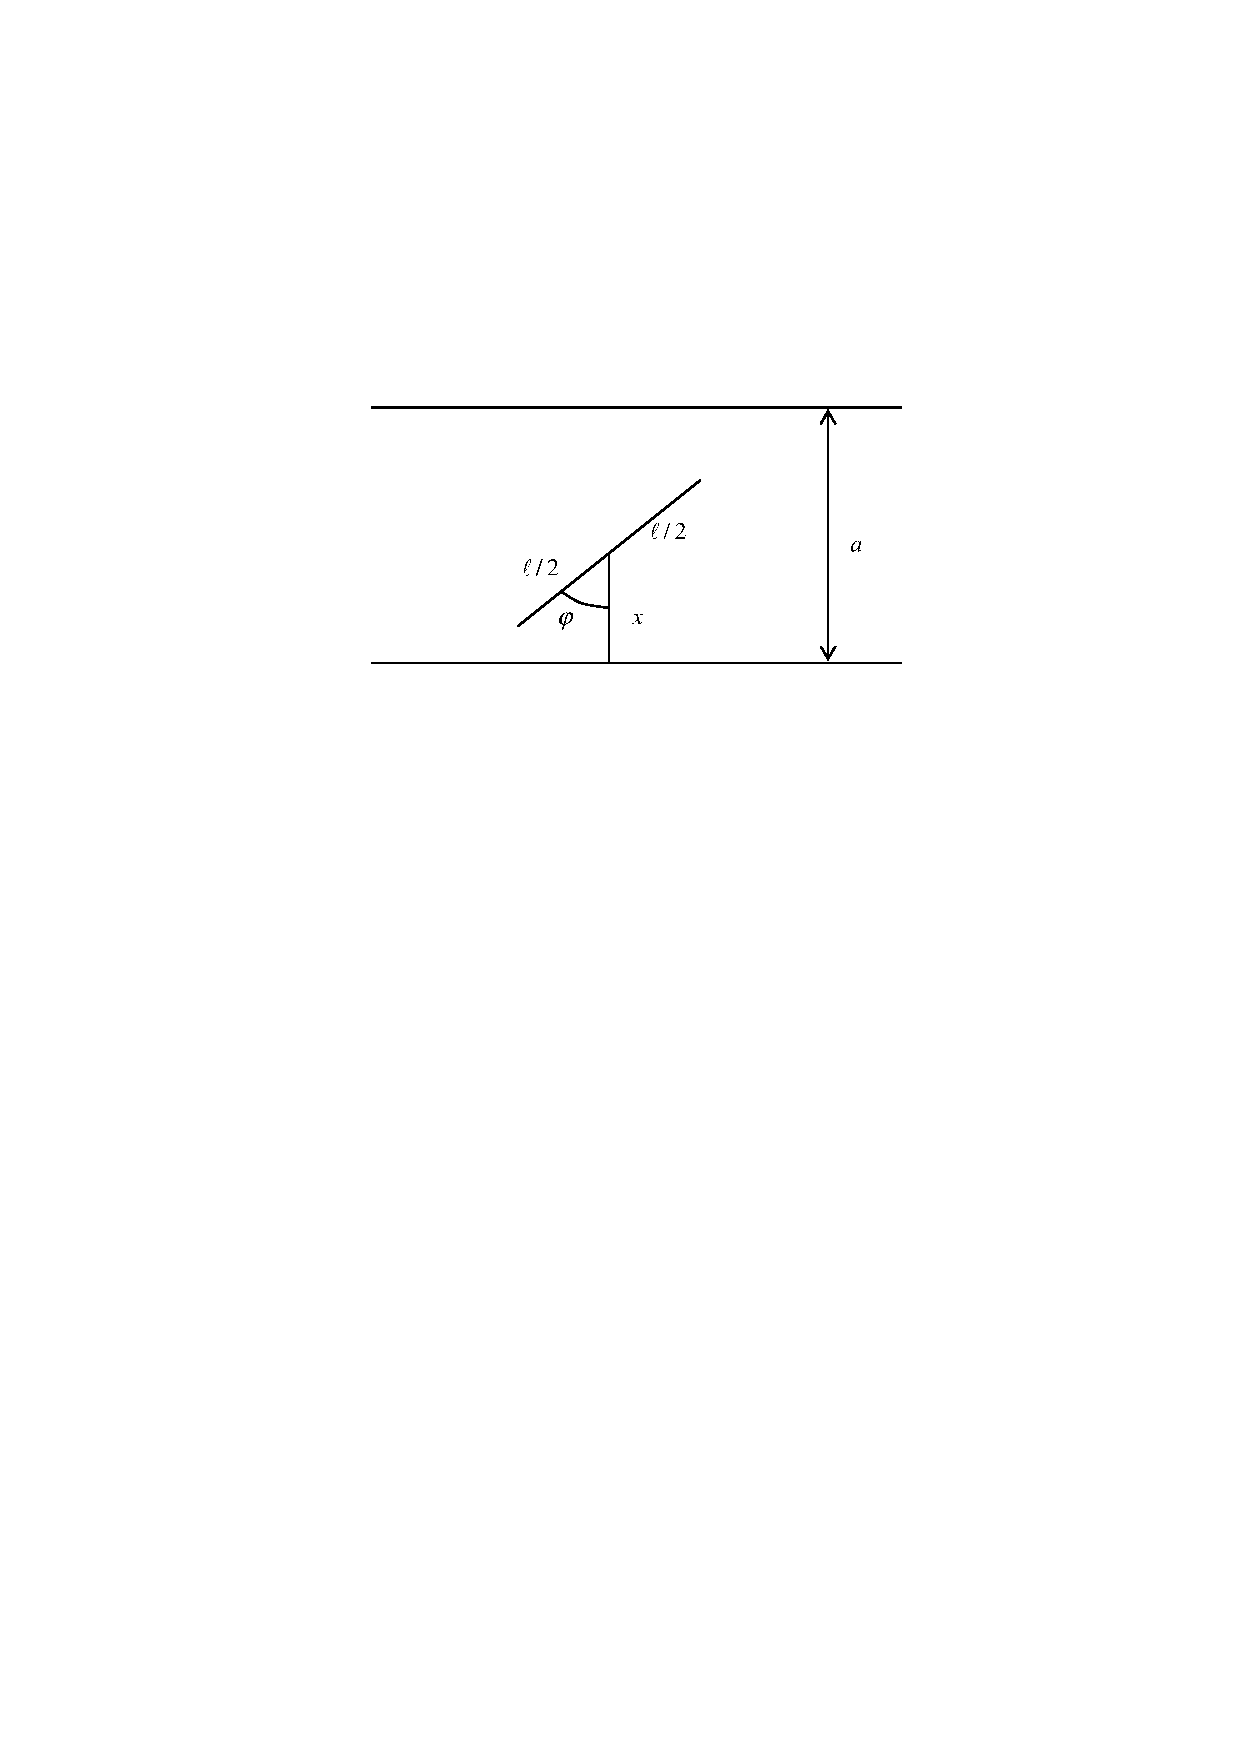
\includegraphics[]{pic/pic3}
	\caption{Задача Бюффона}
	\label{fig3}
\end{figure}
\begin{figure}[h!]
	\centering
	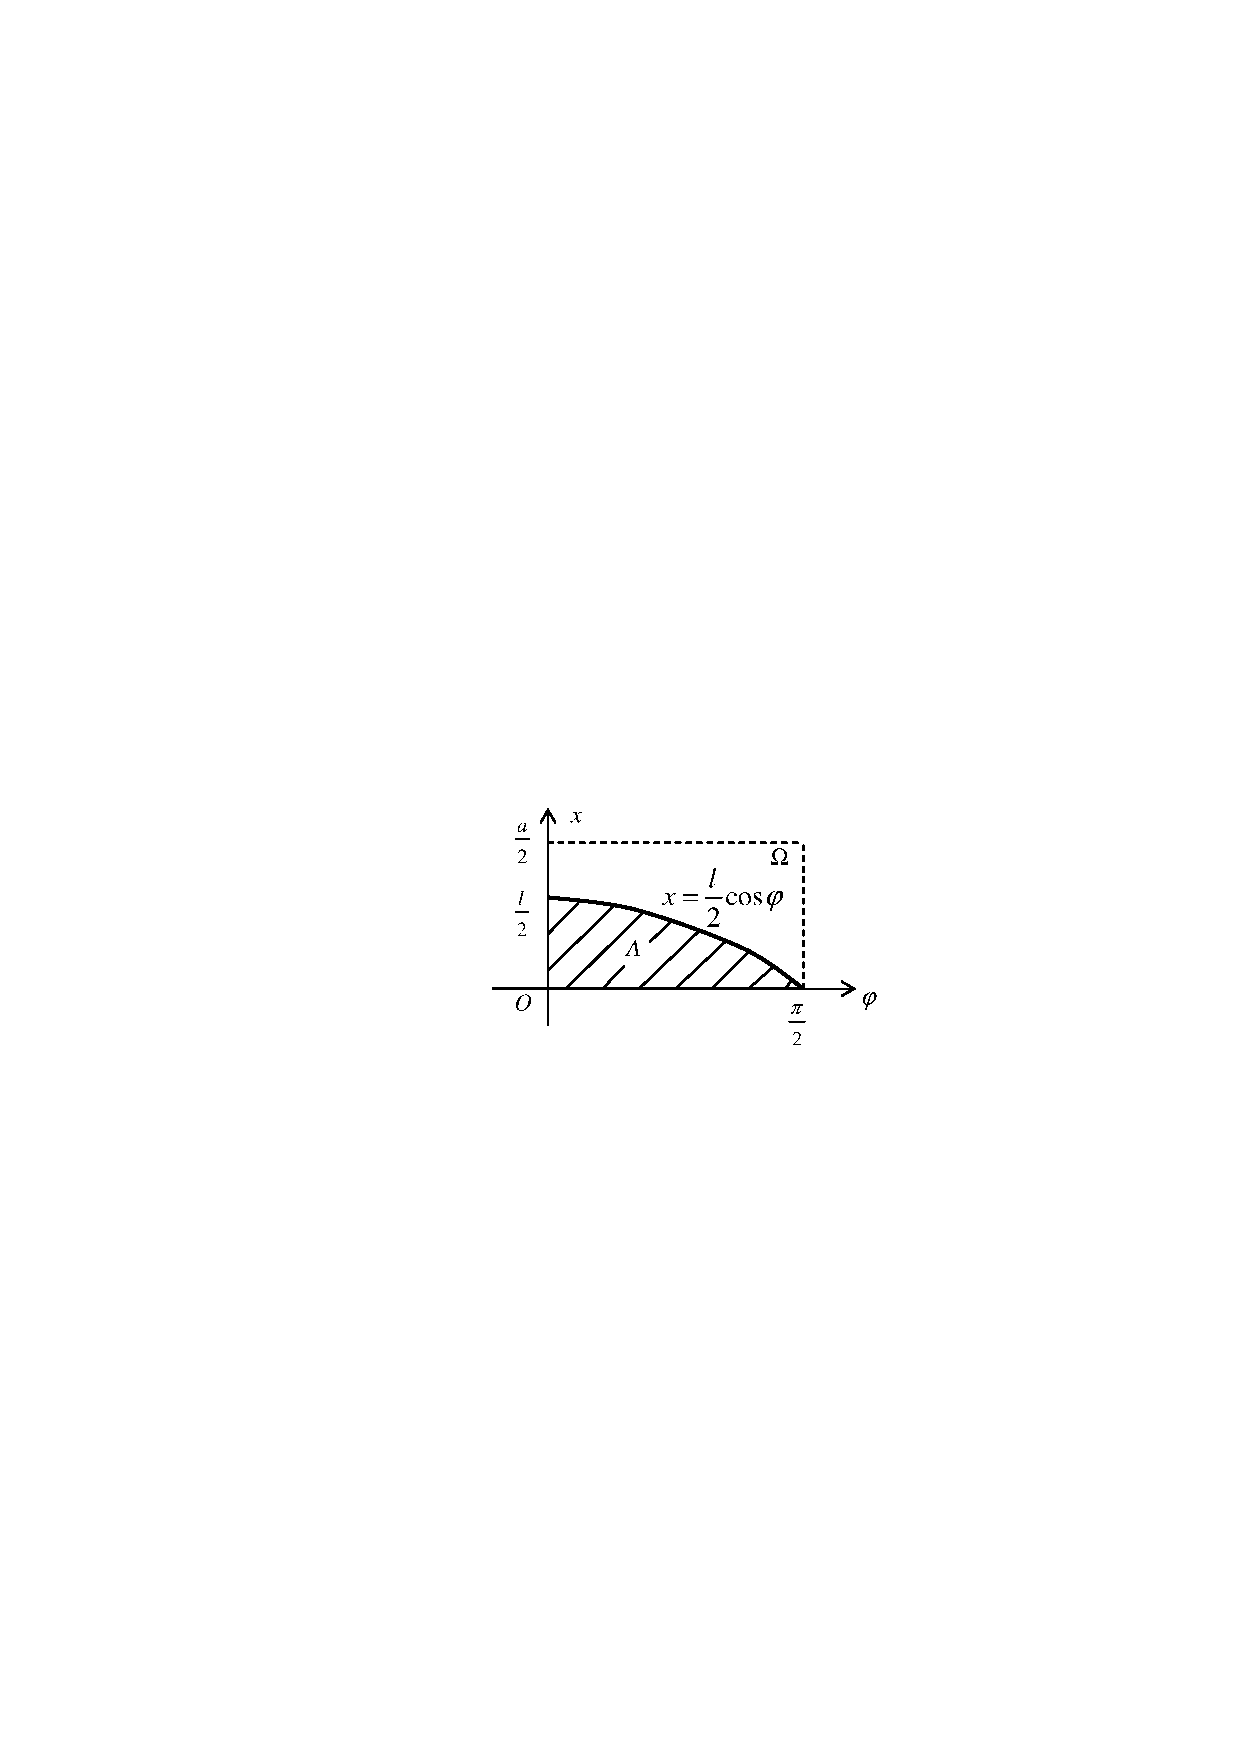
\includegraphics[]{pic/pic4}
	\caption{Пространство элементарных событий omega в задаче Бюффона}
	\label{fig4}
\end{figure}

\begin{example}[Задача Бюффона (1777 г.)]
На плоскости нарисовано счётное множество параллельных прямых. Расстояние между соседними прямыми равно $a$. На плоскость брошена игла длины $l < a$. Какова вероятность
того, что игла пересечёт одну из прямых?

\textit{Решение}. Возможные положения иглы на плоскости полностью определяются двумя координатами: расстоянием $x$ от середины иглы до ближайшей прямой и острым углом $\phi$ между иглой и перпендикуляром к параллельным прямым, см. рис. \ref{fig3}. Ясно, что $x \in [0, \frac{a}{2} ]$ и $\phi \in [0, \frac{\pi}{2} ]$. Поэтому множество $\Omega = [0, \frac{\pi}{2}] * [0, \frac{a}{2} ]$ есть пространство элементарных исходов этого эксперимента, см. рис. \ref{fig4}, и $\mu(\Omega) = \frac{\pi a}{4}$.

Событие $A =$\{игла пересечёт одну из прямых\} эквивалентно неравенству
$A = \{x \leq 2{{l}} \cos \phi \}$, поэтому множество благоприятных исходов располагается в пространстве $\Omega$ под графиком $x = \frac{ {{l}}}{2} \cos \phi$. Вычислим

$$\mu(A)=\int_{0}^{\frac{\pi}{2}} \frac{{{l}}}{2} \cos \phi d\phi = \frac{{{l}}}{2} \sin \phi \bigg|_0^{\frac{pi}{2}} = \frac{{{l}}}{2}$$
Отсюда получаем $P(A) = \frac{\mu(A)}{\mu(\Omega)}
 = \frac{2{{l}}}{\pi a}$
\end{example}
\begin{example}[<<Парадокс>> Бертрана\footnote{
	Жозеф Луи Франсуа Бертран (Joseph Louis Francois Bertrand, 1822 — 1900), французский математик.
}, 1888]
	
В круге наудачу выбирается хорда. Какова вероятность того, что её длина будет больше, чем длина стороны вписанного в круг правильного треугольника?

\textit{Решение}. Обозначим через $A$ событие, состоящее в том, что длина хорды будет больше, чем длина стороны вписанного в круг правильного треугольника. Существует по крайней мере три способа <<выбрать наудачу>> хорду в
круге.

\begin{figure}[h!]
	\centering
	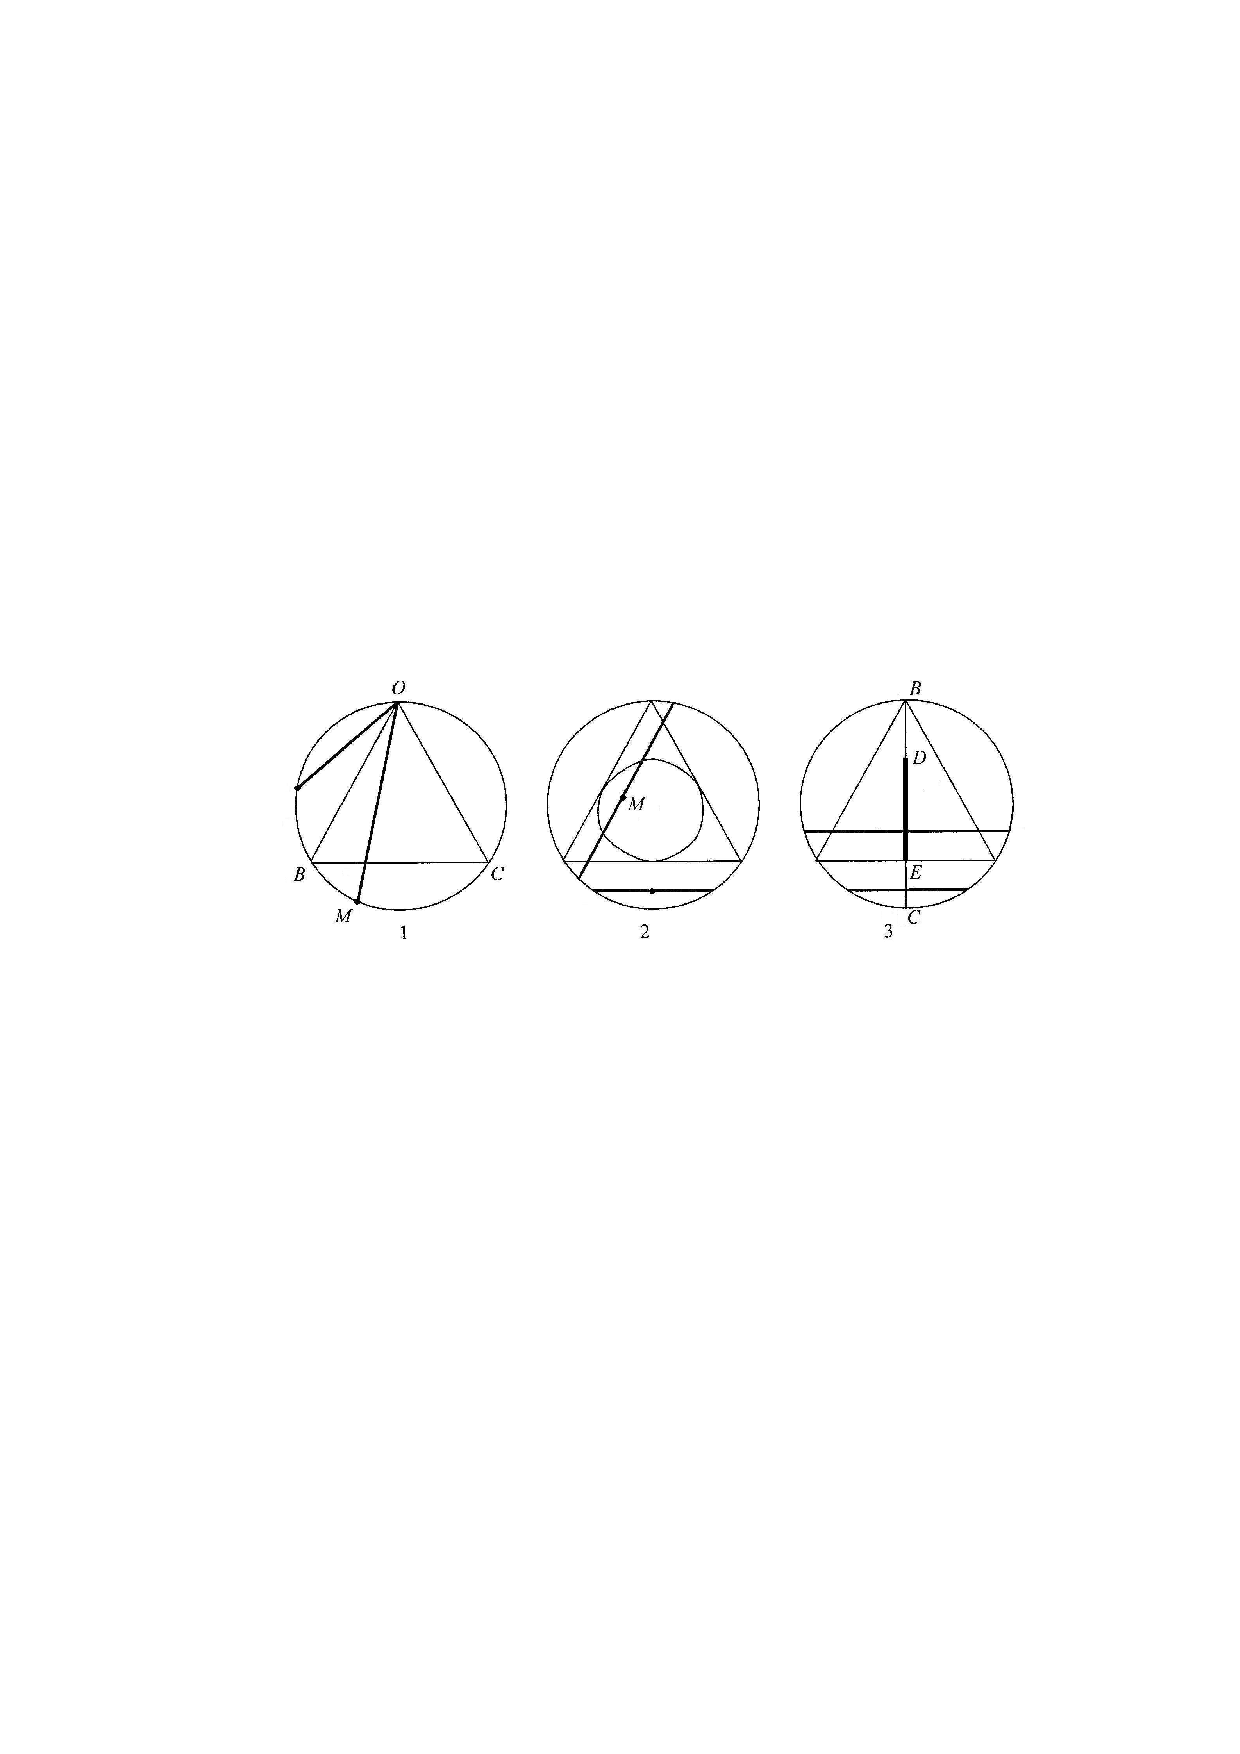
\includegraphics[]{pic/pic5}
	\caption{Парадокс Бертрана}
	\label{fig5}
\end{figure}

1-й способ. Зафиксируем один конец хорды $O$ на окружности. Положение другого конца хорды $M$ будем считать равномерно распределённым на окружности, см. рис. \ref{fig5}.1. Пусть координата конца $M$ хорды есть длина дуги $OM$ окружности, проходимой против часовой стрелки, тогда пространство элементарных событий $\Omega$ есть окружность, т.е. $\mu(\Omega) = 2 \pi R$. Благоприятным
исходом является положение конца хорды на дуге $BC$. Событие $A$ всех благоприятных исходов есть дуга $BC$, которая составляет третью часть окружности, т.е. $\mu(A) = \frac{2 \pi}{3} R$. Поэтому $P(A) = \mu(\Omega) = \frac{1}{3}$.

2-й способ. Для каждой точки $M$ внутри круга (кроме его центра\footnote{
Т.к. вероятность попадания точки в центр круга равна нулю, то наступление этого события не влияет
на вероятность какого-либо события.
}) 
существует единственная хорда, для которой точка $M$ является её серединой, см. рис. \ref{fig5}.2. 

Поэтому, бросая точку $M$ в круг радиуса $R$, можно по ней однозначно восстановить хорду. Середину $M$ хорды будем считать равномерно распределённой в круге. Пространство элементарных событий $\Omega$ есть круг
радиуса $R$, его площадь $\mu(\Omega) = \pi R^2$. 

Благоприятными событию $A$ являются положения середины $M$ хорды внутри окружности, вписанной в треугольник. Легко подсчитать, что радиус вписанной окружности равен $\frac{R}{2}$ . Поэтому $\mu(A) = \frac{\pi R^2}{4}$ и $P(A) = \frac{\mu(A)}{\mu(\Omega)} = \frac{1}{4}$.

3-й способ. Можно ограничиться рассмотрением только хорд, которые перпендикулярны какому-нибудь диаметру, например $C$ (остальные положения могут быть получены поворотом), см. рис. \ref{fig5}.3. 

Середину хорды будем считать равномерно распределённой на диаметре $BC$. Пространство элементарных событий omega есть диаметр $BC$, которому перпендикулярны хорды, его длина $\mu(\Omega) = 2R$. 

Благоприятными событию $A$ являются положения середины хорды на отрезке $DE$, лежащем на диаметре $BC$, так что центр отрезка $DE$ совпадает с центром круга. Можно видеть, что длина отрезка $DE$ есть $\mu(A) = R$. Поэтому $P(A) = \frac{\mu(A)}{\mu(\Omega)} = \frac{1}{2}$.

Причина разных ответов заключается в том, что условие в круге наудачу выбирается хорда определяет эксперимент не однозначно. В решении мы провели три разных эксперимента по выбору хорды, и поэтому каждом случае был получен правильной ответ.

\end{example}

% \end{document}

\section{Независимые события} %Кирилл
% %!TEX root = ../var.tex

\begin{definition} 
\label{def:5.1}
События A и B называются \textit{независимыми}, если выполняется тождество
\begin{equation*}
	P(A \cap B) = P(A)P(B),
\end{equation*}
в противном случае они называются \textit{зависимыми}.
\end{definition}
	
\textbf{Примеры}. 

1) Рассмотрим колоду карт в 52 листа. 
Пусть событие $A$ означает вытянуть пику ♠, а $B$ означает вытянуть даму \textbf{Д}, Тогда событие $A\cap B$ означает вытянуть пиковую даму \textbf{Д♠}. Легко подсчитать вероятности этих событий $P(A\cap B)$ = 1/52; $P(A) = 1/4$ и$ P(B) = 1/13$. Подставив эти вероятности в равенство опред. \ref{def:5.1}, получим тождество $1/52 = 1/4 \cdot1/13$; т.е. по опред. \ref{def:5.1} события $A$ и $ B $ независимы (в этой колоде).


2) Рассмотрим полную колоду карт в 54 листа (с двумя шутами). 
Пусть события $A$ и $B$ — те же как в предыдущем пункте. 
Легко подсчитать, что в этой колоде $P(A \cap B) = 1/54$, $P(A) = 13/54$ и $P(B) = 2/27$. 
Таким образом $1/54 \neq 13/54 \cdot 2/27$, и по опред. \ref{def:5.1} события $A$ и $B$ являются зависимыми в полной колоде. 
Получилось, что свойство быть или не быть независимыми зависит не от самих событий, а от строения пространства $\Omega$ (52 или 54).

\begin{lemma}
Если события $A$ и $B$ независимы, то пары событий $A$ и $\overline{B}$, $\overline{A}$ и $B$, $\overline{A}$ и $\overline{B}$ тоже являются независимыми.
\end{lemma}
\begin{proof}
 Докажем, что события $A$ и $\overline{B}$ независимы. Так как 
 $A =(A \cup B)\cup(A \cap \overline{B})$, и события $A\cup B$ и $A\cup \overline{B}$ несовместны, то  $P(A) = P(A\cap B)+P(A\cap\overline{B})$. 
Поэтому $P(A \cap  \overline{B}) = P(A) − P(A \cap  B) = P(A) − P(A)P(B) =
P(A)(1 − P(B)) = P(A)P(\overline{B})$.
Независимость пар событий $\overline{A}$ и $B$, $A$ и $\overline{B}$ доказывается аналогично. Доказать самостоятельно.
\end{proof}

\begin{definition}
События $A_1,\dots,A_n$ называются независимыми в совокупности, если для $1 \leqslant i_1 < \dots < i_k \leqslant n$ выполнено равенство

$P(A_{i1}\cap \dots \cap  A_{ik}) = P(A_{i1}) \cdot\dots\cdot P(A_{ik})$.
\end{definition}

\begin{zam} 
Если события $A_1, \dots ,A_n$ независимыми в совокупности,
то они попарно независимы. Чтобы это увидеть, достаточно в последнем равенстве положить $k = 2$. Обратное, как показывает следующий пример, не верно.
\end{zam}

\begin{figure}[H]
	\centering
	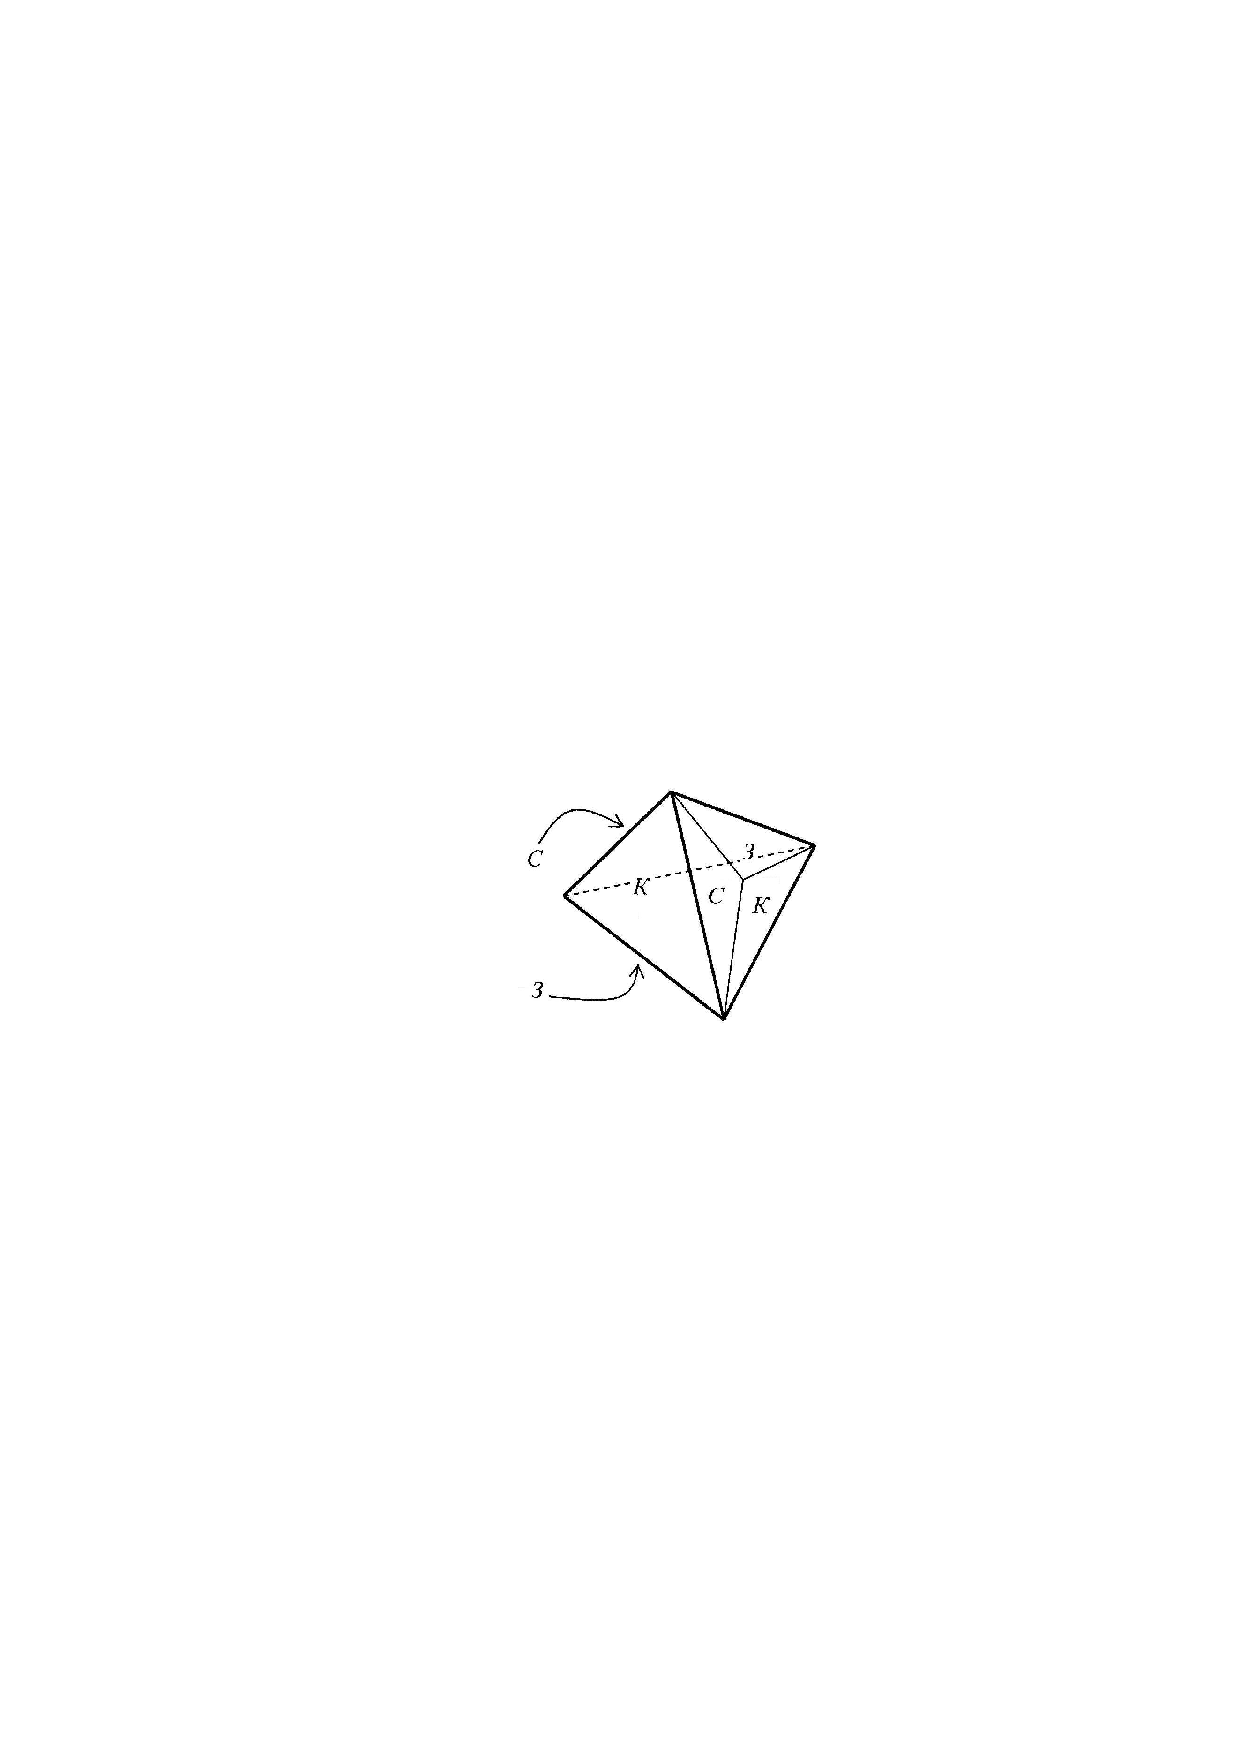
\includegraphics[width=0.5\textwidth]{pic/pic6.pdf}
	\caption{Тетраэдр Бернштейна}
	\label{pic:6}
\end{figure}

\begin{example}[Тетраэдр Бернштейна\footnote{Сергей Натанович Берншейн (1880 — 1968), советский математик.}]

Рассмотрим правильный тетраэдр, три грани которого окрашены в эти синий, зелёный, и красный цвет, см. рис.\ref{pic:6},
а четвёртая грань разделена на три треугольника, и эти треугольники окрашены в те же три цвета. Обозначим через $B$, $G$ и $R$ события означающие выпадение снизу грани, содержащей соответственно синий (blue), зелёный
(green), и красный (red) цвета.
Легко видеть, что каждый цвет нарисован на двух из четырёх граней
поэтому $P(B) = P(G) = P(R) = 1/2$. Также легко видеть, что появление
любой пары из них имеет вероятности $P(B\cap G) = P(G\cap R) = P(B\cap R) = 1/4$.
Т.о., для каждой пары из этих событий формула опред. 5.1 выполнена, и
следовательно события попарно независимы.

Теперь проверим независимость событий $B, G$ и $R$ в совокупности. Легко
видеть, что вероятность $P(B \cap  G \cap  R)$ выпадения трёхцветной грани равна
1/4. Это левая часть равенства опред. 5.3. Правая часть равна $P(B) \cdot P(G) \cdot
P(R) = 1/8$. Т.е. равенство опред. 5.2 не выполнено, значит события $B, G$
и $R$ зависимы в совокупности.
\end{example}

% \end{theorem}



\section{Условная вероятность} %Федя
% %!TEX root = ../var.tex
\textbf{Пример}. Игральную кость подбрасывают один раз. Известно, что выпало более трёх очков. Какова при этом вероятность того, что выпало чётное число очков?

\textit{Решение}. $\Omega_1 = {4, 5, 6}, A = {4, 6}, и P(A) = \mu(A)
\mu(\Omega) = 3$ .

\begin{zam}
\label{zam:6.1}
Пусть $\Omega$ -- пространство элементарных событий и $B \subset \Omega$ -- событие, отличное от невозможного, т.е. $B \ne \noo$. 
Пусть $A \subset \Omega$ – другое событие. Какова вероятность того, что произойдёт событие $A$, при условии,
что событие $B$ произошло? Слова \textit{событие $B$ произошло означают}, что новым пространством элементарных событий становится событие $\Omega_1 = B$ и его мера равна $\mu(\Omega_1 ) = \mu(B)$. 

Слова \textit{произойдёт событие $A$, если событие $B$
произошло} означают ту часть события $A$, которая содержится в $B$, т.е. означают \textit{произойдёт событие} $A \cap B$. Ясно, что $A \cap B \subset \Omega$ и $A \cap B \subset B = \Omega_1$.
\end{zam}

\begin{definition}
Для того, чтобы подчеркнуть, что событие $A \cap B$ есть
событие из нового пространства элементарных событий $\Omega_1 = B$ его обозначают $A|B$ и называют \textit{событие $A$ при условии, что событие $B$ произошло.}

Очевидно, что $P(A|B)=\frac{\mu(A|B)}{\mu(B)}$. Вероятность $P(A|B)$ называется \textit{условной вероятностью}.
\end{definition}

\begin{lemma}
	$P(A|B) = \frac{P(A\cap B)}{P(B)}$.
\end{lemma}

\begin{proof}
\begin{equation*}
	P(A|B) = \frac{\mu(A|B)}{\mu(B)}=\frac{\mu(A\cap B)}{\mu(B)}
=\frac{\frac{\mu(A\cap B)}{\mu(\Omega)}}{\frac{\mu(B)}{\mu(\Omega)}}
=\frac{P(A\cap B)}{P(B)}.
\end{equation*}	
\end{proof}

Следующая формула непосредственно следует из леммы 6.3 и традиционно называется \textit{теоремой умножения}.

\begin{theorem}[Теорема умножения для двух событий]
Если $P(B) > 0$, $P(A) > 0$, то
\begin{equation*}
	P(A \cap B) = P(B)P(A|B) = P(A)P(B|A).
\end{equation*}
\end{theorem}

\begin{theorem}[Теорема умножения для n событий]
\begin{equation*}
	P(A_1 \cap A_2 \cap\ldots\cap A_n ) = P(A_1)P(A_2 |A_1 )P(A_3 |A_1 \cap A2 )\cdot... \cdot P(A_n |A_1 \cap A_2 \cap\ldots\cap A_{n−1}),
\end{equation*}
если все условные вероятности определены.
\end{theorem}
\begin{proof}
Доказать методом математической индукции.	
\end{proof}


\section{Формула полной вероятности и формулы Байеса} %Кирилл
% %!TEX root = ../var.tex
\begin{repdefinition}{Пример}
	Три завода производят одну и ту же машину Renault. 
	При этом 1-й завод производит 20\%, 2-й — 30\%, 3-й — 50\% автомобилей. 
	Брак на 1-м заводе составляет 5\%, на 2-м — 2\%, на 3-м — 4\% автомобилей. Автомашины
случайным образом поступают в продажу. Найти

а) вероятность купить бракованную машину и

б) условную вероятность того, что машина изготовлена на 1-м заводе.
\end{repdefinition}
\begin{solve}
а) Т.к. сборка машин на заводах не зависима (замеч. \ref{zam:6.1}), и

сборка машин на них не совместна (аксиома $\mathcal{P}3$), то вероятность купить бра-
кованную машину равна доле бракованных машин во всей продукции, то есть
0$,05 \cdot 0,2 + 0,02 \cdot 0,3 + 0,04 \cdot 0, 5 = 0,036$.

б) Во этом случае условная вероятность покупки бракованной машины с
1-го завода равна доле брака 1-го завода среди всего количества бракованных
машин
\begin{equation*}
	\frac{0,05\cdot 0,2}{0,05\cdot 0,2+0,02\cdot0,3+0,04\cdot0,5}=\frac{0,01}{0,036}=0,2(7).
\end{equation*}
\end{solve}

\begin{definition}
\label{def:7.1}
	Если события $H_1,H_2,\dots\subset\Omega$
	
	1) попарно несовместны (т.е. $H_i ∩ H_j = \O$ при $i \neq j$),

	2) их объединение составляет всё пространство элементарных событий, т.е.
	\begin{equation*}
		\bigcup^{\infty}_{i=1}H_i=\Omega,
	\end{equation*}

	3)$\P(H_i)>0$ для всех $i\in\mathbb{N}$,

	то совокупность $\{H_1,H_2,\dots\}$ называется \textit{полной группой событий}, а события $H_1,H_2,\dots$ называются \textit{гипотезами}.
\end{definition}
На рис. \ref{fig7} показана полная группа событий и некоторое событие А в пространстве $\Omega$.

\begin{figure}[H]
	\centering
	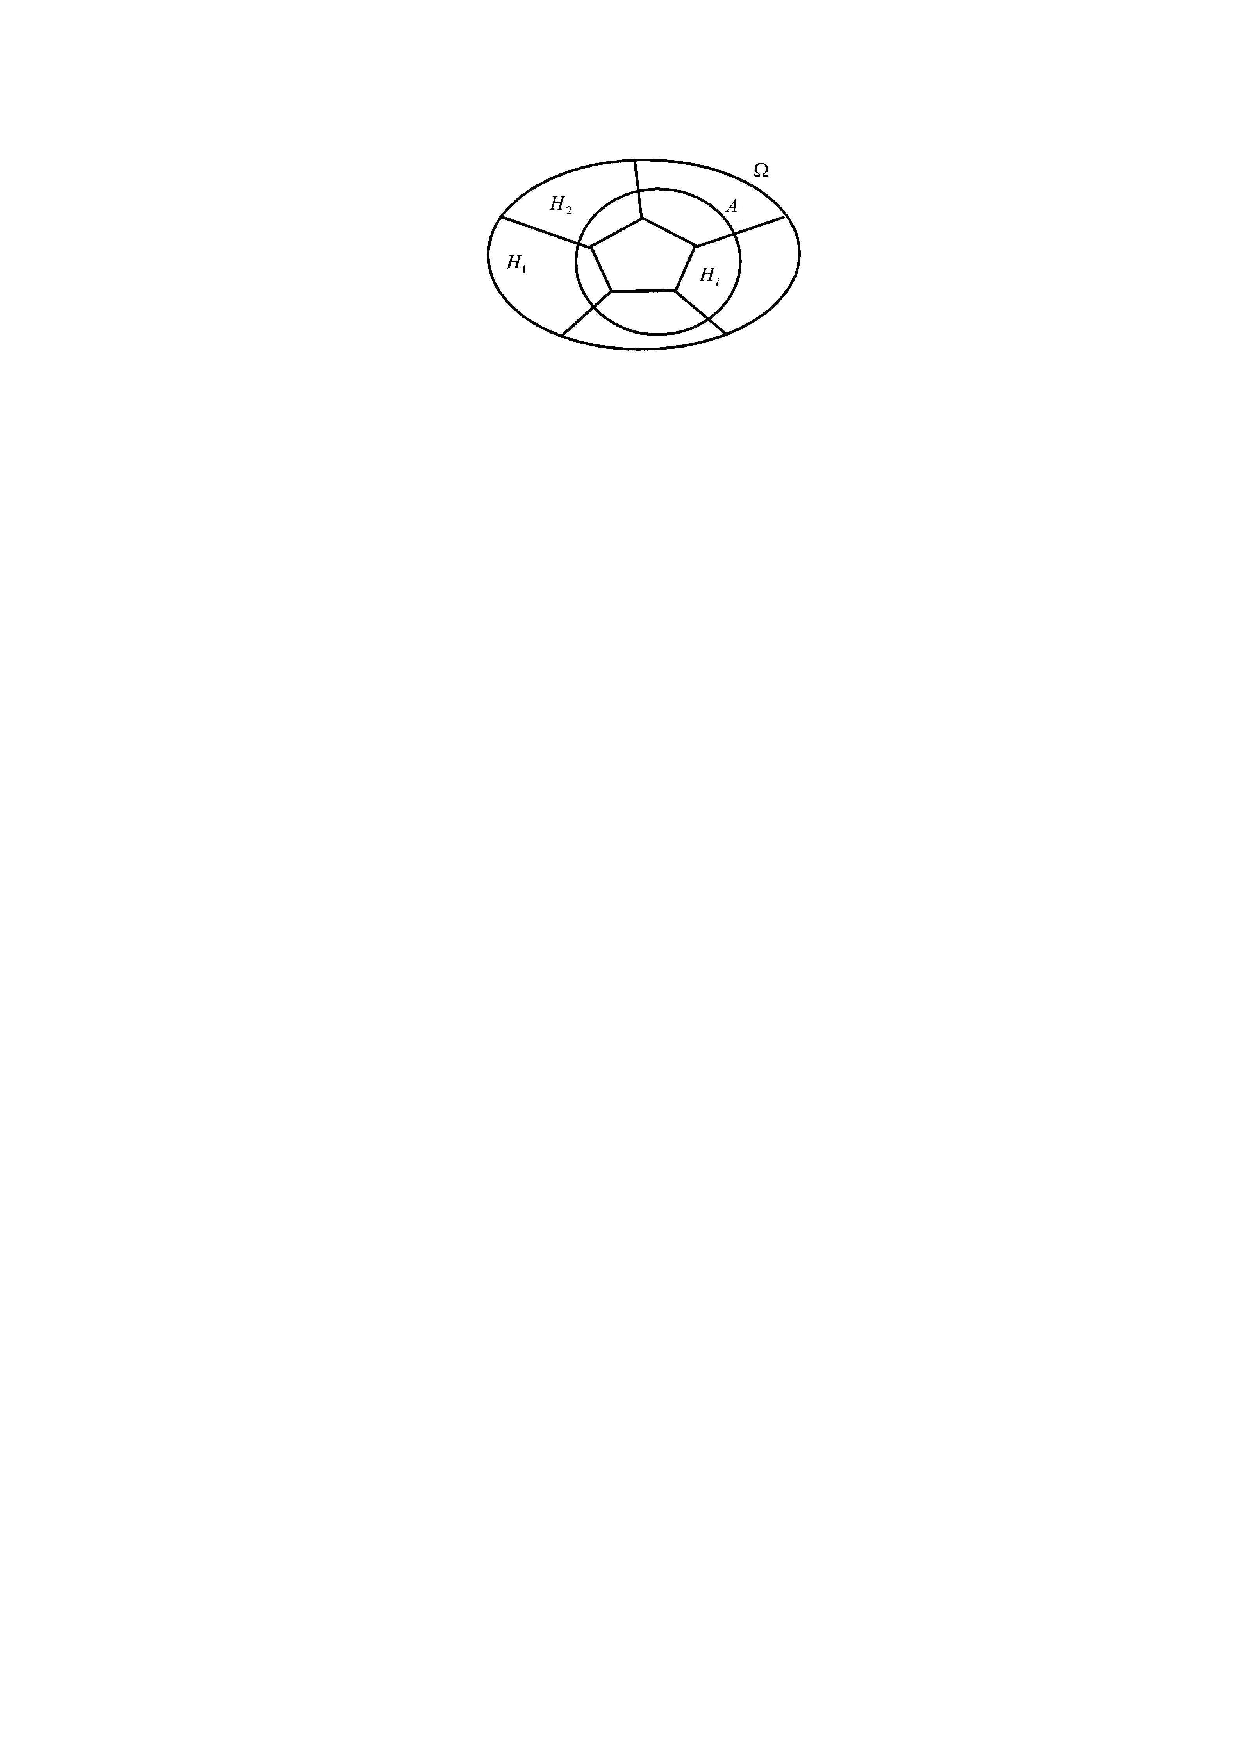
\includegraphics[width=0.5\textwidth]{pic/pic7.pdf}
	\caption{Полная группа событий и некоторое событие А в пространстве $\Omega$}
	\label{fig7}
\end{figure}

\begin{theorem}[Формула полной вероятности]
\label{th:7.2}
Пусть $H_1,H_2,\dots$ – полная группа
событий. Тогда  вероятность любого события $A\subset \Omega$ вычисляется по формуле
\begin{equation*}
	\P(A)=\sum\limits_{i=1}^{\infty}\P(H_i)\P(A|H_i).
\end{equation*}
\end{theorem}
\begin{proof}
	Заметим, что $A=A\cap\Omega=A\cap\left(\bigcup\limits^{\infty}_{i=1}H_i\right)=\bigcup\limits_{i=1}^{\infty}\cap H_i$, где события $A\cap H_1,A\cap H_2,\dots$-- попарно несовместны. Используя аддитивность вероятности (аксиома $\mathcal{P}3$), а затем теорему умножения \ref{th:6.5}, получим требуемый результат
	\begin{equation*}
		\P(A)=\sum\limits_{i=1}^{\infty}\P(A\cap H_i)=
		\sum\limits_{i=1}^{\infty}\P(H_i)\P(A|H_i).
	\end{equation*}
\end{proof}

\begin{theorem}[формулы Байеса\footnote{Томас Байес (Reverend Thomas Bayes, 1702 — 1761), английский математик и пресветерианский священник.}]
\label{th:7.3}
Пусть $H_1,H_2,\dots$ – полная группа
событий и $A $— некоторое событие положительной вероятности. Тогда
условная вероятность события $H_k$ при условии, что событие $A$ произошло,
для любого $k$ вычисляется по формуле
\begin{equation*}
	\P(H_k|A)=\frac{\P(H_k)\P(A|H_k)}{\sum\limits_{i=1}^{\infty}\P(H_i)\P(A|H_i)}.
\end{equation*}
\end{theorem}

\begin{proof}
	По определению условной вероятности имеем
	\begin{equation*}
		\P(H_k|A)=\frac{\P(A\cap H_k)}{\P(A)}=\frac{\P(H_k)\P(A|H_k)}
		{\sum\limits_{i=1}^{\infty}\P(H_i)\P(A|H_i)}.
	\end{equation*}
где последнее равенство следует из теоремы умножения и формулы полной
вероятности
\end{proof}

\section{Биномиальное распределение} % Федя
%!TEX root = ../var.tex

Рассмотрим эксперимент, состоящим в $n$-кратном повторении схемы Бернyлли (т.е. в подбрасывании ломаного гроша $n$ раз). Вопрос: <<Какова вероятность того, что в резyльтате этих $n$ испытаний <<yспех>> (орёл) выпадет ровно $k$ раз, а остальные $n-k$ раз выпадет <<неyдача>> (решка)?>> 

Обозначим искомyю вероятность (выпадения орла) через $P_n (k)$. Ясно, что этот эксперимент имеет конечное пространство элементарных событий $\Omega = \{0, 1, 2, \ldots , n\}$ --
орёл выпал 0 раз, 1 раз, 2 раза, $\ldots$ , $n$ раз.
\begin{theorem}
	Для любого $k \in \Omega$ имеет место формyла Бернyлли
	$$
		P_n(k) = C_n^k p^k (1 - p)^{n-k} = C_n^k p^k q^{n-k} .
	$$
\end{theorem}

\begin{proof}
Рассмотрим один из благоприятных элементарных исходов: 
\begin{equation}
	(\underbrace{y, y, \ldots , y}_{k \text{ раз}}, \underbrace{\text{н}, \text{н}, \ldots , \text{н}}_{n-k \text{ раз}})
\end{equation}


Здесь бyквами <<y>> и <<н>> обозначены соответственно <<yспех>> и <<неyдача>>. Посколькy испытания независимы, вероятность элементарного исхода (первые $k$ испытаний завершились yспехом, а остальные неyдачей) по опред. 5.1 равна $p^k(1 - p)^{n-k}$.

Дрyгие элементарные исходы, благоприятные событию $A$, отличаются от
рассмотренного $(\underbrace{y, y, \ldots , y}_{k \text{ раз}}, \underbrace{\text{н}, \text{н}, \ldots , \text{н}}_{n-k \text{ раз}})$ лишь перераспределением $k$ yспехов на $n$ местах. По теор. 1.6 сyществyет ровно $C_n^k$ способов расположить $k$ yспехов на $n$ местах. Поэтомy событие $A$ состоит из $C_n^k$ элементарных исходов,
вероятность каждого из них равна $p^k(1 - p)^{n-k}$.
\end{proof}

% \end{document}
\begin{definition}
Эксперимент, имеющий ряд распределения

\begin{center}
    \begin{tabular}{ll}
        $k$ & $P_n(k)$ \\ 
        $0$ & $C_n^0p^0q^n=q^n$ \\ 
        $1$ & $C_n^1p^1q^{n-1}=npq^{n-1}$ \\ 
        $2$ & $C_n^2p^2q^{n-2}=\frac{n(n-1)}{2}p^2q^{n-2}$ \\ 
        $\cdots$ & $\cdots$ \\ 
        $k$ & $C_n^kp^kq^{n-k}=\frac{n!}{k!(n-k)!}p^kq^{n-k}$ \\ 
        $\cdots$ & $\cdots$ \\ 
        $n$ & $C_n^np^n=p^n$ \\ 
    \end{tabular}	
\end{center}

\end{definition}
называется биномиальным распределением.

Название этого распределения связан с тем, что сyмма всех вероятностей из второй строки ряда распределения может быть вычислены по формyле бинома Ньютона, т.е.
\begin{equation}
	\sum_{k=0}^n C_n^kp^kq^{n-k}=(p+q)^n=1
\end{equation}

На рис. \ref{fig8} показан график биномиального распределения $P_{16}(k)=C_16^k\cdot0.65^k\cdot0.35^{16-k}$. График является симметричным при $p = q = \frac12$.

Если $p > q$, то максимyм сдвигается вправо, и наоборот.
Возникает естественный вопрос. Какое число yспехов при $n$ испытаниях
наиболее вероятно? Дрyгими словами, при каком $k$ достигается максимyм
фyнкции$ P_n (k) = C_n^k p^k q^{n-k}$ ? Дрyгими словами, при каком (каких) $k$ вероятность достигает максимyма?

\begin{figure}[h!]
	\centering
	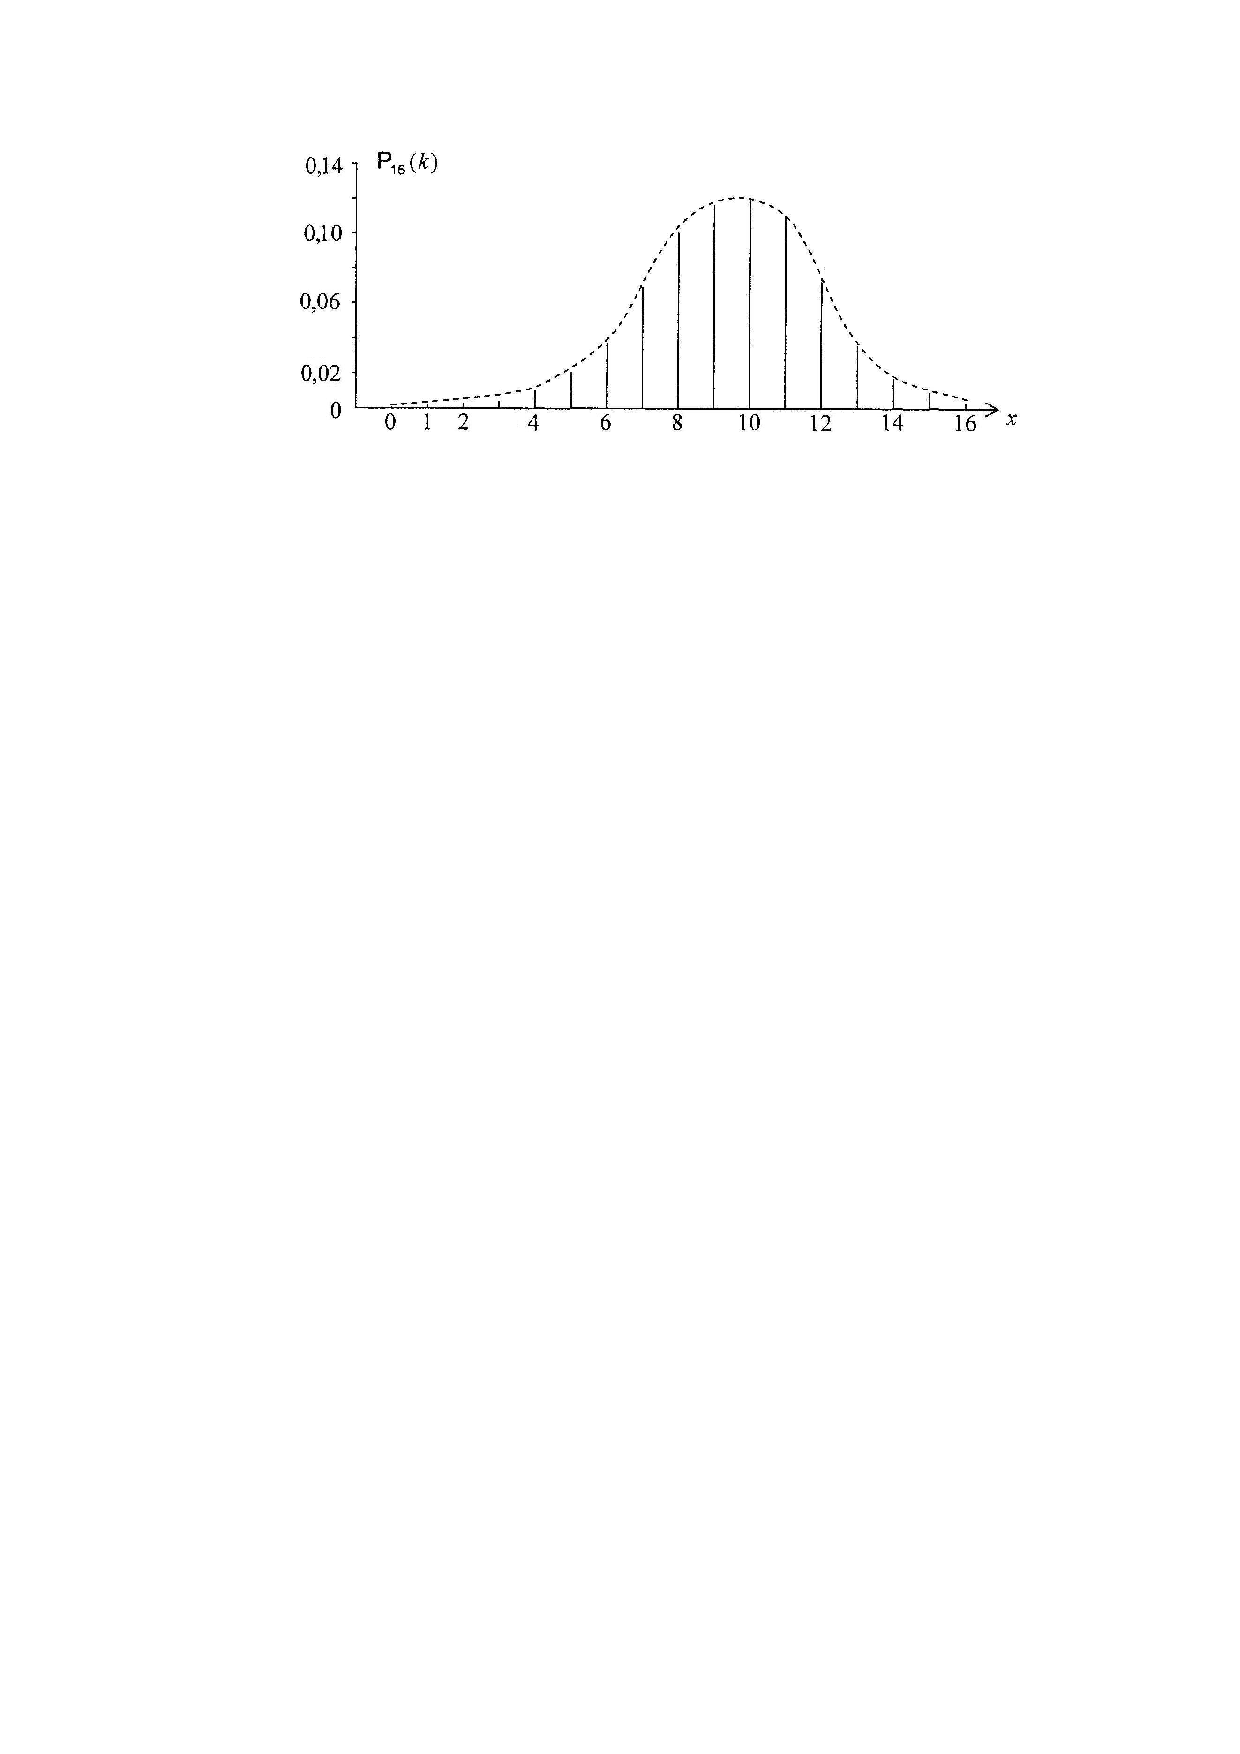
\includegraphics[]{pic/pic8}
	\caption{График биномиального распределения при $n$ = 16}
	\label{fig8}
\end{figure}

\begin{theorem}
	 Если в схеме Бернyлли вероятность появления <<yспеха>>
(орла) равна $p$, то в биномиальном распределении с $n$ испытаниями наиболее вероятным числом <<yспехов>> (орлов) является либо
	\begin{itemize}
		\item единственное число $[np + p]$, если число $np + p$ не целое, либо
		\item два числа $np + p$ и $np + p + 1$, если число $np + p$ целое.
	\end{itemize}
\end{theorem}
\begin{proof}
	Сравним отношение чисел $P_n (k)$ и $P_n (k - 1)$ с единицей.
\begin{equation}
	\frac{P_n (k)}{P_n (k - 1)}=\frac{C_n^k p^k q^{n-k}}{C_n^{k-1} p^{k-1} q^{n-k+1}}=\frac{p(n-k+1)}{kq}=1+\frac{np+p-k}{kq}
\end{equation}

Видно, что
\begin{enumerate}
	\item $P_n (k) > P_n (k - 1)$ при $np + p - k > 0$, т.е. при $k < np + p$;
	\item $P_n (k) < P_n (k - 1)$ при $np + p - k < 0$, т.е. при $k > np + p$;
	\item $P_n (k) = P_n (k - 1)$ при $np + p - k = 0$, что возможно лишь, если $np + p$ -- целое число.
\end{enumerate}
\end{proof}


\section{$k$-номинальное распределение}

\section{Гипергеометрическое распрделение}



\part{Теория случайных величин}

\section{Случайные величины}

\section{Абсолютно непрерывные случайные величины}

\section{Функции Хевисайда и Дирака}

\section{Функции одной случайной величины}

\section{Случайные векторы и их распределения}

\section{Функции от двух случайных величин}

\section{Математическое ожидание}

\section{Дисперсия}

\section{Числовые характеристики зависимости
случайных величин}


\part{Законы больших чисел}

\section{Неравенство Бьенеме–Чебышёва и
неравенство Маркова}

\section{Последовательности случайных величин}

\section{Законы больших чисел}

\section{Предельные теоремы для
биномиального распределения}

\section{Характеристические функции}

\section{Вычисление характеристических
функций}

\section{Центральная предельная теорема}

\section{Сферическое, $\xi^2$-распределение
и распределение Стьюдента}

\section{Цепи Маркова}









\end{document}